%% 
%% ACS project dissertation template. 
%% 
%% Currently designed for printing two-sided, but if you prefer to 
%% print single-sided just remove ",twoside,openright" from the 
%% \documentclass[] line below. 
%%
%%
%%   SMH, May 2010. 


\documentclass[a4paper,12pt,twoside,openright]{report}


%%
%% EDIT THE BELOW TO CUSTOMIZE
%%

\def\authorname{From Context Embeddings to Meaning Embeddings \xspace}
\def\authorcollege{David Yenicelik \\ ETH Zürich\xspace}
\def\authoremail{yedavid@ethz.ch}
\def\dissertationtitle{}
\def\wordcount{14,235}


%\usepackage[dvips]{epsfig,graphics} 
\usepackage{epsfig,graphicx,verbatim,parskip,tabularx,setspace,xspace}
\usepackage{amsmath, amsfonts}
\usepackage{bbm}
\usepackage{amsfonts}
\usepackage{siunitx}
\usepackage{caption}
\usepackage{subcaption}
\usepackage{empheq}
\usepackage{float}


\usepackage[ruled,vlined]{algorithm2e}
\usepackage{tabularx,booktabs}


%% START OF DOCUMENT
\begin{document}


%% FRONTMATTER (TITLE PAGE, DECLARATION, ABSTRACT, ETC) 
\pagestyle{empty}
\singlespacing
% title page information
\begin{titlepage} 

\begin{center}
\noindent
\huge
\dissertationtitle \\
\vspace*{\stretch{1}}
\end{center}

\begin{center}
\noindent
\huge
\authorname \\
\Large
\authorcollege      \\[24pt]

\includegraphics{CUni3.eps}
\end{center}

\vspace{24pt} 

\begin{center}
\noindent
\large
{\it A dissertation submitted to the University of Cambridge \\ 
in partial fulfilment of the requirements for the degree of \\ 
Master of Philosophy in Advanced Computer Science} 
\vspace*{\stretch{1}}
\end{center}

\begin{center}
\noindent
University of Cambridge \\
Computer Laboratory     \\
William Gates Building  \\
15 JJ Thomson Avenue    \\
Cambridge CB3 0FD       \\
{\sc United Kingdom}    \\
\end{center}

\begin{center}
\noindent
Email: \authoremail \\
\end{center}

\begin{center}
\noindent
\today
\end{center}

\end{titlepage} 

\newpage
\vspace*{\fill}

\onehalfspacing
\newpage
{\Huge \bf Declaration}

\vspace{24pt} 

I David Yenicelik of ETH Zürich, being a candidate for the M.Sc. ETH in
Computer Science, hereby declare that this report and the
work described in it are my own work, unaided except as may be
specified below, and that the report does not contain material that
has already been used to any substantial extent for a comparable
purpose.

\vspace{24pt}
Total word count: \wordcount

\vspace{60pt}
\textbf{Signed}: 

\vfill

This dissertation is copyright \copyright 2020 David Yenicelik. 
\\
All trademarks used in this dissertation are hereby acknowledged.



\newpage
\vspace*{\fill}

\singlespacing
\newpage
{\Huge \bf Abstract}
\vspace{24pt} 

One of the goals of Natural Language Understanding \textit{NLU} is to formalize written text in a way, such that linguistic features can be captured through computational models, which can then again be used for downstream machine learning tasks.
The most popular methodology in NLU is the use of vectors that represent written text, including word-vectors, sentence-vectors, etc. 
These vectors are often referred to as \textit{embedding} vectors, as they embed more complex concepts into a vector representation.

Because embeddings - due to their strong usage in downstream tasks - can be considered as the fundamental unit of machine learning in the domain of natural language, any shortcomings will influence the performance of the target task.
Given that language models such as BERT only capture a black-box function $f$ between input and output, our aim is to understand how the subspace organization relates to linguistic features.
We focus our analysis on \textit{semantics}, which captures a meaning within language, as this is one of the most important features of language. 
We analyse the BERT language model, as it provides a good balance between popularity, close to state-of-the-art performance, and generalizability to other modern language models.
\\

Our main contributions are the following: (1) We test for linear separability and ability to partition the space into semantic clusters within the sampled BERT vectors.
We show that while linear separability is possible, it is nearly impossible to find modes in the data which correspond to semantic classes that are as cleanly as defined by WordNet.
We conclude that BERT organized the embedding vectors imminently by context, and very little by semantics alone.
This can easily introduce undesirable properties such as strong sentiment, leading to considerable bias in downstream tasks.
(2) We analyze the relationship between part-of-speech and semantics. 
We show that these show a strong correlation in languages and that modern language models capture this strong correlation.
This affects the conclusion of some related work which had analysed language models which capture semantics, but which did not account for the correlation between part-of-speech and semantics.
(3) Finally, we introduce additional parameters for words whose sampled embedding vectors have high variance over the embedding space.
We investigate what downstream tasks are most affected  and use this as a proxy to understand what information is captured the most by the directions with high variance. \\

\newpage
\vspace*{\fill}


\pagenumbering{roman}
\setcounter{page}{0}
\pagestyle{plain}
\tableofcontents
\listoffigures
\listoftables

\onehalfspacing

% Definition of macros
\newcommand{\norm}[1]{\left\lVert#1\right\rVert}
\newcommand{\bracket}[1]{\left[#1\right]}
\newcommand{\absdet}[1]{\left|#1\right|}
\newcommand{\bftab}{\fontseries{b}\selectfont}
%% START OF MAIN TEXT 

%\chapter{Introduction}
\chapter{Introduction}

%TODO Re-do this part
\pagenumbering{arabic} 
\setcounter{page}{1} 

\newpage
\chapter{Motivation}
 
- Natural Language Understanding (NLU) lies in the intersection of formalising human text into a computer-readable format.
- Computer-readble units must be numerical, thus we represent words and meanings by vectors
- The relationships between vectors should cover underlying relations between the word meaning
- Language models are a generalization of word vectors
- Word embeddings such as Word2Vec and language models such as BERT are used for other tasks, which are refered to as "downstream" tasks, due to their nature of using up these word-embeddings and language models

- Because these are the most basic units of text, any shortcomings and properties will propagate over to any downstream task
- Some properties include that static word vectors like word2vec form a bijection between discrete vectors and word tokens. 
However, because a single word can entail multiple meanings, such as the polysemous word "bank" ( (1) financial instution, (2) a sitting bench ), this results in a lossy compression
- Other language models like context embeddings entail too much information, and also include other linguistic features such as semantic information, relatenedness to unrelated concepts.
These properties can easily introduce bias into any downstream tasks.
- We conjecture that many language tasks incl. translation will benefit most from meaning information

- Our general approach is to start with a complex language model that outputs context embeddings, and find signals / vectors that entail meaning.
- Although this work is dedicated to the domain of natural language understanding, the principles analysed in this work should generalize to other domains with similar structural properties as well, where we want to denoise some embedding space to some select properties.


%\chapter{Background} 
\chapter{Background} 

TODO: Take some more from here
%TODO http://da.inf.ethz.ch/teaching/2019/CIL/lecture/CIL2019-05-Word-Embeddings.pdf

- Some of the main points behind \cite{harris54} are that there is inherent structure in language, and that this structure can be formalized.
- \cite{harris54} mentions that the relation between the linguistic representation in terms of sounds and tokens are related to the meaning that the representation entail.
- However, despite the obvious relationship, the distinction between distributional structure of the language and meaning is not always clear. and that there is a "parallel" meaning structure, and argues that there is not a one-to-one relation between vocabulary and classification of meaning. 
- Also argues that the meaning of a word is entailed by it's environment, and the words that it occurs with.
- Other viewpoints (CITE HOFMANNs "teachers") In the end, language captures the evolution of human thought.

- cite paper "meaning is classified by its context"

Chronologically, the following data structures are manifestations of the above idea of defining a word by it's neighbourhood.

\section{Linguistic Features}
Polysemy:
a word may have multiple meanings.
in a cross-lingual embedding space, this feeling is amplified.
there's some work in multi-sense embedding.
this should enable to capture more fine-grained embeddings embeddings.

Over the past decades, linguists have tried to inject structure into language. 
Similar to features in machine learning, there are properties in language. 
There is a vast number of linguistic features, going from phonological features, morphological and syntactic features to semantic features.
To keep this analysis concise, we will give a short introduction of what features that are relevant for the topic of finding suitable word embeddings.

\paragraph{Lexical features} include word classes, such as nouns, verbs and adjectives, which follow certain grammatical rules in western languages.
Whenever we are looking to parse for such lexical features, we use the python spaCy package \cite{spacy}.
As defined in \cite{spacyb}, some of the linguistic features that are available to us include but are not limited to

\begin{enumerate}
\item adjectives \textit{ADJ}
\item adposition \textit{ADP}
\item adverbs \textit{ADV}
\item auxiliary \textit{AUX}
\item conjunction \textit{CONJ}
\item coordinating conjunction \textit{CCONJ}
\item determiner \textit{DET}
\item interjection noun \textit{INTJ}
\item noun \textit{NOU}
\item numeral \textit{NUM}
\item particle \textit{PART}
\item pronoun\textit{PRON}
\item proper noun \textit{PROPN}
\item punctuation \textit{PUNCT}
\item subordinating conjunction \textit{SCONJ}
\item symbol \textit{SYM}
\item verb \textit{VERB}
\end{enumerate}

These features can alter as we look at different languages
%TODO turn this into a multi-column table

\paragraph{}

\section{Word Embeddings}

\paragraph{Word-Embeddings}
In general, we want to find a mapping 

\begin{equation}
w^t \mapsto (x_w, b_w) \in \mathcal{X}^{d + 1}
\end{equation}{\label{map:embedding_mapping}}

where $w^t$ is a token representation from a vocabulary $w^t \in V$ and where this token representation is transformed into a $d$-dimensional vector representation $x_w$, and a bias-term $b_w$ that is specific to the token $w^t$.
Whenever we will talk about \textit{word-vectors}, \textit{(word)-embeddings}, or \textit{feature-vectors}, we will refer to the image of the above map. 
For convenience and unless stated otherwise, we will assume that $x_w$ absorbs the bias term $b_w$ as an additional vector-element.
Also, for simplicity and unless otherwise stated, we will use the euclidean real-valued vector-space $mathbb{R}^{d+1}$ to described the resulting embedding vectors.
Please note, however, that the choice of the embedding space $\mathcal{X}$ is not fixed in general, and as such, work in other spaces have also been conducted. 
%TODO Cite Gerry


\paragraph{Distance} Now our goal is to build an embedding space where the relationship between words are meaningful.
Specifically, we want to incorporate the notion of \textit{meaning} into these word-embeddings, which should follow following properties.
Formally, we introduce the concept of \textit{distance} $d : \mathcal{X}  \times \mathcal{X} \mapsto [ 0, \inf )$, which should capture the relation between different elements. 
For a set of elements $x, y, z \in \mathcal{X}$, following properties must hold for our distance metric to be a valid on:

\begin{enumerate}
\item $d(x, y) \geq 0$ (non-negativity)
\item $d(x, y) = 0 \iff x = y$ (identity, i.e. if two embedding vectors are identitical, they must capture the same underlying word instance)
\item $d(x, y) \leq d(x, z) + d(z, y)$ (triangle inequality)
\end{enumerate}{\label{def:distance}}

One consequence of the above rules is that for words $a, b, c$, each having a word embedding $x, y, z$ respectively, $d(x, y) < d(x, z) \iff $ word instance $b$ is conceptually closer to word $a$ than word $c$.
For convenience, whenever I input $a, b, c$ into the distance function $d$, the word-embeddings for the corresponding word-tokens shall be used.
Also, please notice that I left out the notion of symmetry for distance measures.

\paragraph{Learning a distance}
Often in machine learning, one wants to maximize a certain probability distribution given some data $\mathbf{X}$.
In the context of word vectors, we want to maximize the probability that $w$ occurs in the context window of $w \prime$ through some parameters $\theta$.
Implicitly, this corresponds to minimizing the distance between $w$ and $w^{\prime}$, while keeping the distance between $w$ and all other words constant. 
We call $w \prime$ a \textit{context word} for $w$.

\begin{equation}
p \left(w | w^{\prime}\right)
\end{equation}

and 

\begin{equation}
\forall w, w^{\prime} : \hspace{20pt} \text{max } p \left(w | w^{\prime}\right) \iff \text{min } d(w | w^{\prime})
\end{equation}

\paragraph{Going from the distributional structure of sentences to learning distances between words.} One of the early formalizations of representing the distributional structure of words through was expressed in \cite{bengio03}, which argues that a sequential statistical model can be constructed to estimate this true posterior.  
In it's most naive form, this would imply that we can estimate the probability of a word $w^{(t)}$ after words $w^{(t-1)}, \ldots, w^{(1)}$ as

\begin{align}
p(\mathbf{w}) &= p(w^{(t)}, \ldots, w^{(1)}) \\
&= p\left( w^{(t)} | w^{(t -1)}, \ldots, w^{(1)} \right)
\end{align}{\label{eq:naive_sequential_probability}}

%TODO check the underlying equation again!!

where $\mathbf{w} = w^{(1)}, \dots, w^{(T)} $ is the sequence of words, $p(\mathbf{w})$ the probability of this sentence occurring.

Because inference for the above equation would have been computationally infeasible, the notion of \textit{n-grams} was introduced to estimate this conditional probability, following a markov assumption.

\begin{align}
p\left( w^{(t)} | w^{(t -1)}, \ldots, w^{(1)} \right) \approx p\left( w^{(t)} | w^{(t -1)}, \ldots, w^{(t - n + 1)} \right)
\end{align}

Often, the above equation will be simplified even further using the independence of words assumption

However, because we are only interested in the distance between two words at a time (and not the full seqence) \cite{bengio03} simplify the above function using the assumption of marginalized independence of words amongst each other w.r.t. a target word $(t)$ (we can do this because we marginalize over all possible combinations of target words and context words).

\begin{equation}
p(\mathbf{w})=\prod_{t=1}^{T} \prod_{\triangle < t} p\left( w^{(t)} | w^{(t -\Delta)}\right)
\end{equation}{\label{eq:naive_sequential_probability}}


 whose probability we wish to estimate (and maximize if this is in the given training dataset), $\mathcal{I}=\{-R, \ldots,-1,1, \ldots, R\}$ is the so-called \textit{context window} which includes all the words that $R$ index units to the left, and $R$ index units to the right of the word of interest $w^(t)$.

\paragraph{However, we do not need to only look at only the previous words}.
One can consider the full neighbourhood of a word.
If we describe this by a loss-measure we would like to minimize, this would result in 

%TODO I guess this is the skip-gram approach, the bag-of-words is again a different one

\begin{equation}
\mathcal{L}(\theta ; \mathbf{w})=\prod_{t=1}^{T} \prod_{\triangle \in \mathcal{I}} p_{\theta}\left(w^{(t)} | w^{(t +\Delta)}\right)
\end{equation}{\label{eq:basic_equation_log_maximization}}

where $\mathbf{w} = w^{(1)}, \dots, w^{(T)} $ is the sequence of words whose probability we wish to estimate (and maximize if this is in the given training dataset), $\mathcal{I}=\{-R, \ldots,-1,1, \ldots, R\}$ is the so-called \textit{context window} which includes all the words that $R$ index units to the left, and $R$ index units to the right of the word of interest $w^(t)$.

%TODO rephrase the structuring of the n-grams. I don't like how it is introduced here

If $p_\theta$ is a parametric function, one can then optimize for the most optimal $\hat{\theta} = \text{argmax}_\theta \mathcal{L}(\theta ; \mathbf{w})$ using a maximum likelihood estimation approach.

In general, one does not necessarily need to interpret $\mathbf{w}$ as a sequence of word-tokens, but can also interpret $w^{(1)}, \ldots, w^{(T)}$ as \textit{n-grams}, which are triplets of n-characters forming a token-unit.
Generally, the definition of a token is open for interpretation. 
We will generally assume that a single word is a token unless otherwise stated.
%TODO Cite some Token Paper!!

Intuitively the above models fllw the idea expressed by \cite{harris54} very well, speaking that the meaning of a word is captured by its neighborhood.
However, the above equations follow a \textit{continuous bag of words } (CBOW) approach.
A continuous-bag-of-words approach is an approach where we want to predict a target word $w^t$ given some context words $w^{\prime}$.
However, it is also possible to follow a \textit{skip-gram} approach.
Here, we want to predict context words $w^{\prime}$ given a target word $w^t$.

\begin{figure}[h]
	\center
  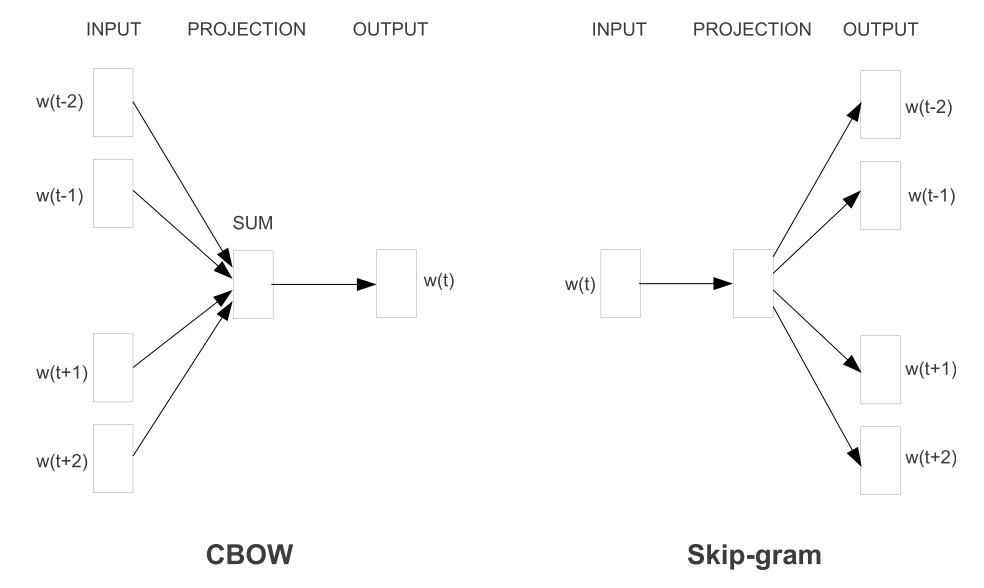
\includegraphics[width=0.6\linewidth]{./assets/background/cbow_and_skipgram.png}
  \caption{Figure taken from \cite{mikolov13}. The CBOW architecture predicts the current word based on the context. The Skip-gram predicts surrounding words given the current word.}
  \label{fig:cbow_skipgram}
\end{figure}

Using a skip-gram approach, \eqref{eq:basic_equation_log_maximization} for example would be reformulated into 
\begin{equation}
\mathcal{L}(\theta ; \mathbf{w})=\prod_{t=1}^{T} \prod_{\triangle \in \mathcal{I}} p_{\theta}\left(w^{(t +\Delta)} | w^{(t)}\right)
\end{equation}{\label{eq:basic_equation_log_maximization_skipgram}}


The question now is, how do we parametrize the distribution $p_\theta(w, w^{\prime})$, as well as the word feature vectors $x_w$ and $b_w$. 
The following will show a few methods of how this can be achieved.
In the following methods shown, we will aim to provide a loss function that we try to minimize, and interesting properties for each method.
However, we will not go into too much details, as to how the loss function is optimized, as almost all of these methods can be solved using gradient-based methods.

\newpage
\subsection{Static Word Embeddings}

Here we will talk about word-embeddings where each word-token only has a single $x_w$. 
Specifically, the mapping \eqref{map:embedding_mapping} is not a probabilistic function with an implicit random factor, but rather a deterministic one.

\subsubsection{Basic Model}

The first model we are going to look at is a most basic model which fulfills the properties of the distance metrics shown in \eqref{def:distance}.

Here, we can introduce a \textit{log-bilinear} model where the log-probability is define as

\begin{equation}
\text{log} p_{\theta}(w | w^{\prime}) = \left\langle\mathbf{x}_{w}, \mathbf{x}_{w^{\prime}}\right\rangle+b_{w} + \text { const. }
\end{equation}

To arrive at the actual probability, we can exponentiate the log-probability as such

$$
p_{\theta}\left(w | w^{\prime}\right)=\frac{\exp \left[\left\langle\mathbf{x}_{w}, \mathbf{x}_{w^{\prime}}\right\rangle+b_{w}\right]}{Z_{\theta}\left(w^{\prime}\right)}
$$

where $Z_{\theta}\left(w^{\prime}\right):=\sum_{v \in \mathcal{V}} \exp \left[\left\langle\mathbf{x}_{v}, \mathbf{x}_{w^{\prime}}\right\rangle+b_{v}\right]$ is a normalization constant such that the probability mass sums to $1$, and the model parameters entail the word-embeddings $\theta = (x_w, b_w) \in \mathbb{R}^{d+1}$

%TODO CIL lecture slides
% http://da.inf.ethz.ch/teaching/2019/CIL/lecture/CIL2019-05-Word-Embeddings.pdf


\subsubsection{Word2Vec}

%TODO look at this more closely again

During training, the above basic model comes with certain drawbacks. The distance would be minimized if all word-embeddings would collapse onto a single point. 
Also, there is no term that forces unrelated words to move away from each other, a property that we are interested in as unrelated words should form embedding vectors that are far from each other.

One of the most prominent example of word vectors manifests itself in the work of \cite{mikolov13} and \cite{mikolov13b}.
Here, a neural network with a single embedding layer can be trained to transform one-hot-vectors $\in \{ 0, 1 \}^{| \mathcal{V} |}$ which represents a word $w$ in vocabulary $\mathcal{V}$
into a latent vector representation $w \in \mathbf{R}^{d + 1}$ using both a continuous bag of word and also a continuous skip-gram approach.
The skip-gram approach is preferred in practice.

Specifically, the loss-function that is optimized looks as follows

\begin{align} 
\mathcal{L}(\theta ; \mathbf{w}) & =\sum_{t=1}^{T} \sum_{\Delta \in \mathcal{I}} [\\ 
& b_{w^{t+\Delta}} +\left\langle \mathbf{x}_{w^{(t+\Delta)}}, \mathbf{x}_{w^{(t)}} \right\rangle \\
& -\log \sum_{v \in \mathcal{V}} \exp \left[\left\langle\mathbf{x}_{v}, \mathbf{x}_{w^{(t)}}\right\rangle+b_{v} \right] 
\end{align}

As one can see, the loss function takes in the bilinear loss from the basic model, and complements this by adding a term, such that random samples are not put next to each other.
This principle is often referred to as \textit{negative sampling}.

\begin{figure}[h]
	\center
  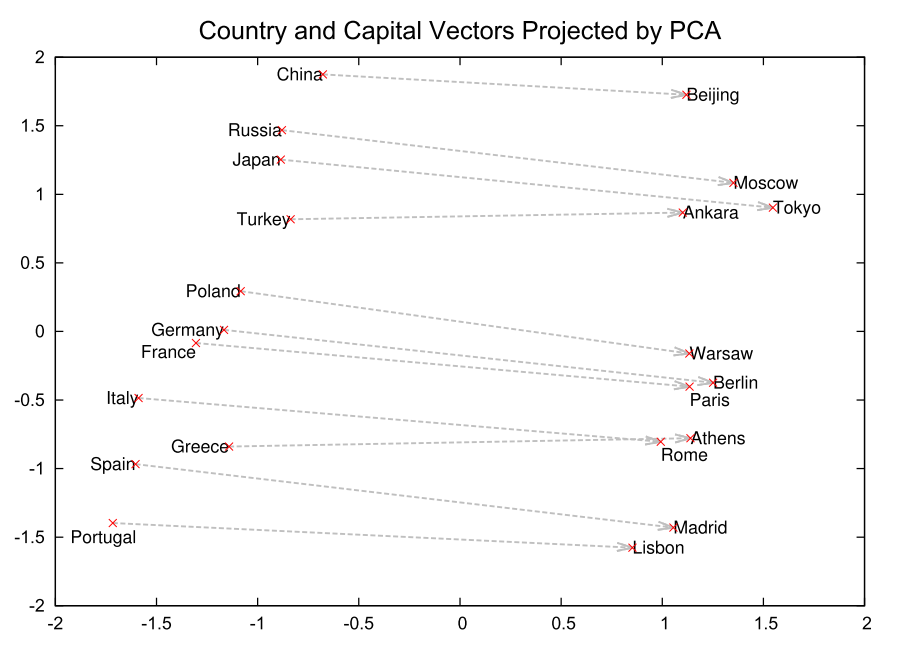
\includegraphics[width=0.6\linewidth]{./assets/background/word2vec_cities.png}
  \caption{Figure taken from \cite{mikolov13b}. A 2-dimensional PCA projection of the 1000-dimensional skip-gram vectors of countries and their capital cities. The proposed model is able to automatically organize concepts and learn implicit relationships between them. No supervised information was provided about what a capital city means.}
  \label{fig:cbow_skipgram}
\end{figure}

%TODO include difference between target vocabulary V and context vocabulary C

\subsubsection{GloVe}

For the global vectors for word representation (GloVe) \cite{pennington14}, the authors follow a more straight-forward matrix factorization approach.

First, a global co-occurence matrix is created $\mathbf{N} = (n_{ij}) \in \mathbb{N}^{|\mathcal{V}| \dot |\mathcal{C}|}$ where each entry $n_{ij}$ is determined by the number of occurrences of word $w_i \in \mathcal{V}$ in context $w_j \in \mathcal{C}$.
Given that the vocabulary size can exceed multiple thousand items, this practically results in a sparse matrix.

\begin{align}
\mathcal{H}(\theta ; \mathbf{N}) &=
\sum_{i, j} f\left(n_{i j}\right)(\underbrace{\log n_{i j}}_{\text {target }}-\underbrace{\log \tilde{p}_{\theta}\left(w_{i} | w_{j}\right)}_{\text {model }})^{2} \\
&= \sum_{i, j} f\left(n_{i j}\right)(\log n_{i j} - \left\langle x_i, y_j \right\rangle )^{2} \\
\end{align}

where $f(n_{ij})$ is the weighting function which assigns a weight for each entry in the co-occurence matrix. 
In the second line, we also again use a bilinear probability density model $\tilde{p}_{\theta}\left(w_{i} | w_{j}\right)=\exp \left[\left\langle\mathbf{x}_{i}, \mathbf{y}_{j}\right\rangle+b_{i}+c_{j}\right]$.
The constants $b_i, c_j$ are left out and are assumed to be absorbed in the embedding vectors.

A popular choice for the weighting function is 

$$
f(n) = \min \left\lbrace 1, \left(\frac{n}{n_{\max}}\right)^{\alpha} \right\rbrace
$$

with $\alpha \in (0, 1]$.
The motivation behind this is that frequent words do not receive a weighting which is "too high" (there is a cutoff at some point) and small counts are considered noise and slowly cancelled out.


\subsubsection{Gaussian Embeddings}

Gaussian Embeddings have been first proposed in the context of words, although prior work has been adapted in embedding matrix-rows into a mean and standard deviation \cite{vilnis14} 

It is a continuous probabilistic relaxation of the otherwise common discrete point vectors.
Each word is represented by a Gaussian distribution in high-dimensional space, with the aim to better capture uncertainty and a representation and it's relationships.
It can also express asymmetric relations more naturally than dot-products or cosine similarity, and enables for better-parametrized rule between decision boundaries.

Training is done using an energy function which is incorporated within a loss function that we try to minimize. 
The energy function describes similarity between two items.
The authors propose the following energy functions to derive a Gaussian word-embedding.

\begin{equation}
L_m(w, c_p, c_n) = max(0, m - E_\theta(w, c_p) + E_\theta(w, c_n)
\end{equation}

Here, $w$ is the word we want to sample, $c_p$ is a "positive" context word, i.e. a word that co-occurs with the word $w$, and $c_n$ is a "negative" context word, i.e. a word that does not co-occur with the word $w$.
Usually the negative context words is sampled randomly from the corpus.
The loss function reminds of a hinge-loss in logistic regression.

The authors propose two possible ways to learn the mean and variance of the Gaussian embeddings.
They argue that the empirical covariance is not the most effective method of deriving the words as Gaussian embeddings.
This does not allow for inclusion between ellipsoids 

\paragraph{Symmetric similarity: expected likelihood or probability product kernel}

We can use any kernel (which is symmetric by definition) to derive at an energy function.
For two Gaussians $f(x)$, $g(x)$, the inner product is defined as:

\begin{align}
E_\theta(w, c) &= \int_{x \in \mathcal{R}^d} f(x)g(x) dx \\
&= \int_{x \in \mathcal{R}^d} \mathcal{N}(x; \mu_w, \Sigma_w) \mathcal{N}(x; \mu_c, \Sigma_c) dx \\
&= \mathcal{N}(0; \mu_w - \mu_c, \Sigma_w + \Sigma_c)
\end{align}

For numerical feasibility and easy of differentiation, we usually maximize the $\text{log} E_\theta(w, c)$ for a given dataset with $w \in \mathcal{W}, c \in \mathcal{C}$.

\paragraph{Asymmetric divergence: KL-Divergence}

We can use more directional supervision to exploit directional supervision, such as a knowledge graph.

Following energy-function is optimized:

\begin{align}
-E(w_i, c_j) & = D_{KL}(c_j || w_i) \\
&= \int_{x \in \mathcal{R}^d} \mathcal{N}(x; \mu_{w_i}, \Sigma_{w_i}) \text{log} \frac{\mathcal{N}(x; \mu_{c_j}, \Sigma_{c_j})}{\mathcal{N}(x; \mu_{w_i}, \Sigma_{w_i})} dx \\
&= \frac{1}{2}\left(\operatorname{tr}\left(\Sigma_{i}^{-1} \Sigma_{j}\right)+\left(\mu_{i}-\mu_{j}\right)^{\top} \Sigma_{i}^{-1}\left(\mu_{i}-\mu_{j}\right)-d-\log \frac{\operatorname{det}\left(\Sigma_{j}\right)}{\operatorname{det}\left(\Sigma_{i}\right)}\right)
\end{align}

Because of the loss function, this can entail information such as "y entails x" as a soft form of inclusion between two datasets (if KL divergence is used).
If a symmetric loss function is used, then this would most likely lead to overlap (IS THIS TRUE...???)

%TODO Veerify this statement again

\paragraph{Uncertainty calculation:} In contrast to the empirical standard deviation as an uncertainty measure, we can now calculate the uncertainty of the inner product (i.e. the distribution $P(z=x^T y)$ using the following formula

\begin{align}
\mu_z = \mu_x^T \mu_y
\Sigma_z = \mu_{x}^T \Sigma_{x} \mu_{x}+\mu_{y}^T \Sigma_{y} \mu_{y}+\operatorname{tr}\left(\Sigma_{x} \Sigma_{y}\right)
\end{align}

We then get an uncertainty bound, where $c$ denotes the number of standard deviations away from the mean.
\begin{equation}
\mu_{x}^{\top} \mu_{y} \pm c \sqrt{\mu_{x}^{\top} \Sigma_{x} \mu_{x}+\mu_{y}^{\top} \Sigma_{y} \mu_{y}+\operatorname{tr}\left(\Sigma_{x} \Sigma_{y}\right)}
\end{equation}

We can learn the parameters $\Sigma$ and $\mu$ for each of these embeddings using a simple gradient-based approach, where we set hard constraints on 

\begin{align}
& \norm{ \mu_i }_2  \leq C, \forall i \\
& m I <  \Sigma_i < M I
\end{align}

The method shows competitive scores to the Skip-Gram model, although usually only with minor improvements depending on the benchmark-dataset.

%TODO Include one part about tokenizers

\newpage
\subsection{Context Embeddings}

Now that we have seen a few methods that aim to capture one embedding $x_w$ for each word-token, we not turn out attention to context embeddings.

Context embeddings are more modern applications of embeddings which 

A single transformer takes as input a sequence $x$ and outputs softmax probabilites.
In the context of sentences, it is able to take as input a full sequence of words.
This has implications for the complexity of the model.
Instead of calculating the raw probability of \eqref{naive_sequential_probability}, and even using a markovian assumption because computation power is expensive, the transformer architecture implicitly calculates the joint probability of an entire sequence of words withouth any explicit conditioning

%TODO: Rephrase this part

\begin{align}
p(w^{(t-d)}) &= p(w^{(t)}, \ldots, w^{(t-d + 1)}, w^{(t-d - 1)}, \ldots, w^{(1)})
\end{align}{\label{eq:transformer_probability}}

where $p(w^{(t-d)})$ is the probability of the target word $w^{(t-d)}$ which we want to calculate.

This modifies our initial ask of calculating $p(w, w^{\prime})$ to not including only a single context word $w^{\prime}$, but rather a wider context \\ (i.e. $w^{(t)}, \ldots, w^{(t-d + 1)}, w^{(t-d - 1)}, \ldots, w^{(1)}$).
Theoretically, and because we want to arrive at some distance measure, $p(w, w^{\prime})$ can still be calculated by marginalizing out all the context-variables except the one of interest.
Specifically, if we are interested in word $w$, we can marginalize out all input words except $w^{\prime}$.
Practically this is infeasible due to the high space, and as such, we make use of some other mechanisms that we will talk about in the "BERT" section below.

%TODO How to marginalize these over?
%TODO Talk about what kind of input these take-in
%TODO Look at bit more closely into the attention mechanism?
%TODO Can draw some more inspiration from this here

Because the following models not merely static word embeddings, but language models, we shall provide a short comparison between for downstream tasks between the individual language models after a short introduction on the details of each language models.

\subsubsection{ELMo}

The simplest idea of context embeddings, which take into account more than just a single word, but all tokens from a predefined context is the \textit{Embeddings from Language Models} (ELMo) model proposed in \cite{peters17}.

In its underlying architecture, ELMo is using LSTMs.
LSTMs are sequential recurrent neural networks .
%TODO how do you best explain LSTMs?

Specifically, LSTMs \cite{hochreiter97} are good at estimating the probability of word $w^{(t)}$ occurring given a previous history of words $w^{(t-1)}, \ldots w^{(1)}$.
In practice, the LSTM is a popular choice for sequence modeling tasks, as it is able to capture very well the following probability distribution.

\begin{equation}
p\left(w_{1},  w_{2}, \ldots, w_{N} \right)=\prod_{k=1}^{N} p\left(w_{k} | w_{k-1}, \ldots, w_{2}, w_{1}\right)
\end{equation}

The ELMo language model now makes use of a backward LSTM, which does not evaluate the probability of a certain token occuring with its \textit{past} words (i.e. the context with context tokens $w^{(k)}$ with $k < t$ for a word $w^{(t)}$ whose probability we want to estimate), but rather considers only the \textit{future context}.
Specifically, this results in 

%TODO Insert an example of what this could look like
\begin{equation}
p\left(w_{1},  w_{2}, \ldots, w_{N} \right)=\prod_{k=1}^{N} p\left(w_{k} | w_{k+1}, w_{k+2}, \ldots, w_{N}\right)
\end{equation}

A bidirectional language model (biLM) combines the above two LSTM models, thus jointly maximizing the log likelihood of the forwards, as well as backward directions.

\begin{align} 
\sum_{k=1}^{N} &\left(\log p\left(w_{k} | w_{k-1}, \ldots, w_{1} ; \Theta_{x}, \vec{\Theta}_{L S T M}, \Theta_{s}\right)\right.\\
+&\left.\log p\left(w_{k} | w_{k+1}, \ldots, w_{N}; \Theta_{x}, \overleftarrow{\Theta}_{L S T M}, \Theta_{s}\right)\right) 
\end{align}

Because the output of a sequential neural network - which the LSTM is part of - includes $2L + 1$ output representations, we receive the following set of vectors, one for each input token, which we now consider the \textit{context embeddings}.
Each context embeddings outputs a vector representing $x_{k}$ for the word token $w^{(k)}$, given its context $ w_{1}, \ldots, w_{k-1}  w_{k+1}, \ldots, w_{N}$.

\begin{align} 
R_{k} &=\left\{\mathbf{x}_{k}^{L M}, \overrightarrow{\mathbf{h}}_{k, j}^{L M}, \overleftarrow{\mathbf{h}}_{k, j}^{L M} | j=1, \ldots, L\right\} \\ &=\left\{\mathbf{h}_{k, j}^{L M} | j=0, \ldots, L\right\} 
\end{align}

Notice that one can stack the above biLM such that the output of one module is taken as input to another module.
The biLM module is stacked twice ELMo.
If a downstream task is trained end-to-end, the all output vectors can be stacked together and provided as input to a final downstrea-specific neural network module.

\subsubsection{The Transformer Architecture}

All of the below presented models use the transformer architecture which initially was presented in \cite{vaswani17}, which shows how far simple \textit{attention} modules can go.

%TODO Go into what attention is

\begin{figure}[h]
	\center
  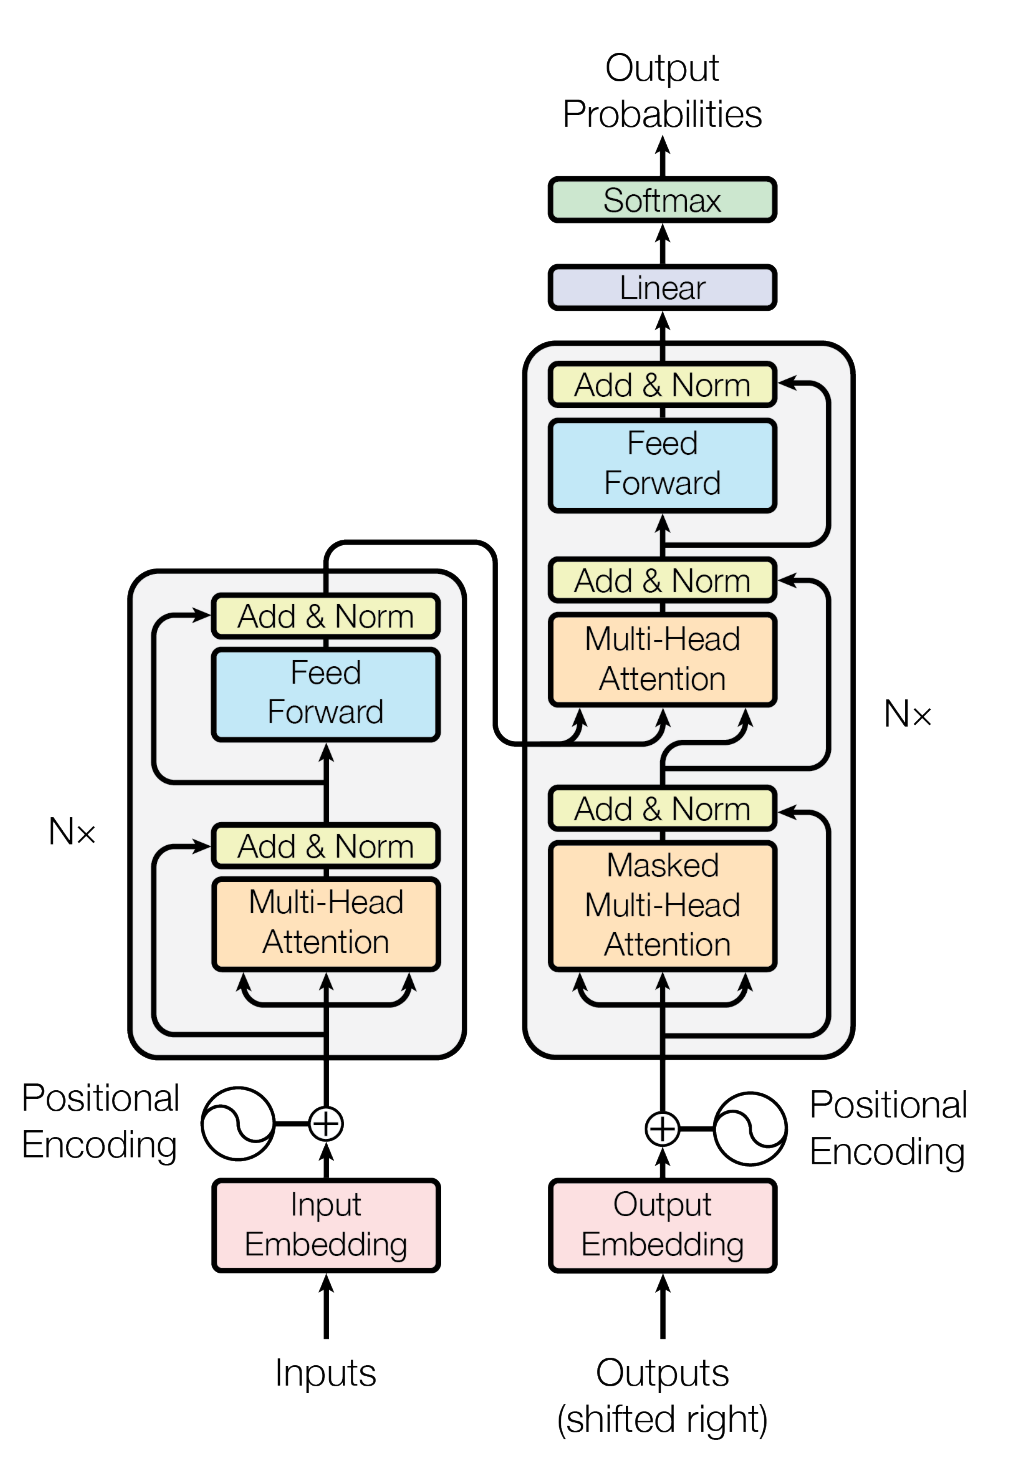
\includegraphics[width=0.4\linewidth]{./assets/background/transformer_module.png}
  \caption{Figure taken from \cite{vaswani17}. The transformer module architecture. The transformer encapsulates multiple attention layers.}
  \label{fig:cbow_skipgram}
\end{figure}



The following architectures are all based on the transformer module.

\subsubsection{BERT}

As introduced in \cite{devlin18}, the Bidirectional Encoder Representations from Transformers model (BERT) combines the above concepts of forward and backwards sequential models with attention, as marked in the transformer architecture above.

\cite{devlin18} argue that the main limitations is that standard language models are unidirection, and that .

BERT introduces itself as a pre-trained language model.
Specifically, it shall be used to fine-tune on specific downstream tasks.

BERT is pre-trained on %TODO 
multiple gigabytes of text .

%TODO talk about masked training

%TODO Talk about tokenizer (wordpiece)

\begin{figure}[h]
	\center
  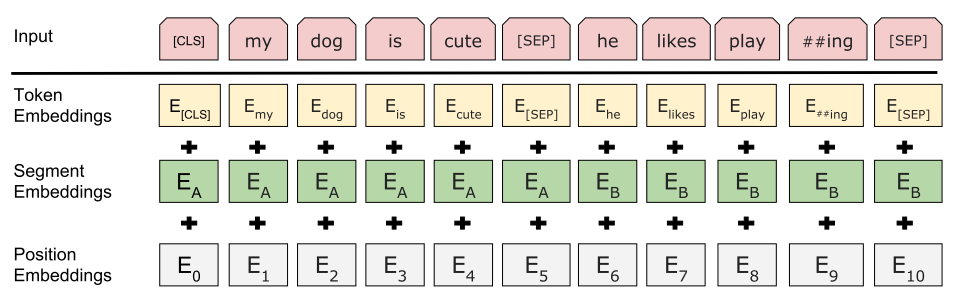
\includegraphics[width=0.6\linewidth]{./assets/background/BERT_multiple_input_tokens.png}
  \caption{Figure taken from \cite{devlin18}. BERT takes as input multiple tokens, including a position embedding, the token embedding and the segment embedding. This allows BERT to distinguish between the location of the word within a sentence, and which word token was provided and which sentence the word token is a part of.}
  \label{fig:cbow_skipgram}
\end{figure}


Multiple versions of BERT are provided, including $BERT_{LARGE}$ which includes %TODO input number of parameters
, and $BERT_{BASE}$ which includes %TODO number of parameters

Ever since BERT came out, a wide variety of similar models came out that mimick the main logic of BERT, and improve upon it, such as DistillBERT \cite{sanh19}.

Numerous works have been published on making BERT representations more compact, for it to be used for on-device text-processing applications, such as more compact sentence-representations \cite{shen19}.



\subsubsection{GPT and GPT-2}

First proposed in \cite{radford18} and further extended in \cite{radford19}.

%TODO read the two papers and take out anything significantly different to BERT.


\subsection{Other methods}

Although the above presented methods are the prevailent methods for word-embeddings, there are also other methods which do not clearly fit into one of the above categories.

\subsubsection{Generating "static" word-embeddings through contextual embeddings}

Some work has been done in extracting word-embeddings from contextual language models like BERT or ELMo.

CITE (BERT WEARS GLOVES: DISTILLING STATIC EMBEDDINGS FROM PRETRAINED CONTEXTUAL REPRESENTATIONS)

(1) Uses \textit{pooling} between BERT tokens to arrive at a single representation between words.

Here, sentences are split by space (tokenized).
Words are tokenized further into a subword as defined by WordPiece (Wu et al. 2016).

The defined pooling operations looks as follows to arrive at the word from the individual subwords:

$$
\mathbf{w}_{c}=f\left(\mathbf{w}_{c}^{1}, \ldots, \mathbf{w}_{c}^{k}\right) ; f \in\{\min , \max , \text { mean, last }\}
$$

where we have subwords $w^{1},  \ldots, w^{k}$ such that $\operatorname{cat}\left(w^{1}, \ldots, w^{k}\right)=w$

Why would any of these pooling operations result in a meaninigful source-word? 
This is just squishing tokens together! \\

-> This is a major limitation for which we may need to use ELMo
-> However this may be needed for "unseen concepts" (which are unseen words...)
-> Perhaps check what fasttext does...?


(2) Uses \textit{context combination} to map from different contexts $c_1, \ldots, c_n$ to a single static embedding $w$ that is agnostic of context.

Proposed are two ways to represent context.

\textbf{Decontextualization} For a single word-context, we siimply feed-in the word by itself to the model.

\textbf{Aggregated} combine $w$ in multiple contexts.
n sentences are sampled from the dictionary $\mathcal{D}$.
From the multiple sampled words, we then apply pooling to arrive at a single representation that aggregates the different tokens into one.

$$
\mathbf{w}=g\left(\mathbf{w}_{c_{1}}, \dots, \mathbf{w}_{c_{n}}\right) ; g \in\{\min , \max , \text { mean }\}
$$


This post extracts (token?) word-embeddings: 
(https://towardsdatascience.com/nlp-extract-contextualized-word-embeddings-from-bert-keras-tf-67ef29f60a7b)

This seems to be a way to extract embeddings for tokens from BERT
(https://github.com/imgarylai/bert-embedding)

(->How can we create a (parametric) probability density from a point-cloud distribution?)

perhaps not necessarily interpretable in standard euclidean space
(https://www.kdnuggets.com/2019/02/bert-features-interbertible.html)
original (https://medium.com/thelocalminima/are-bert-features-interbertible-250a91eb9dc)

Perhaps we can mask all but the target token to arrive at one vector per token (and then combine them somehow...).
But how do they extract the singular word-embeddings...?

(-> you could be like "acquiring bedeutung" is a big problem in many tasks. especially useful when we try to map one concept to another. we look at the NLP task for concreteness)

Generally, really good critique on this paper:

(https://openreview.net/forum?id=SJg3T2EFvr)

usually, we have sentence-embeddings, and do not look at word-embeddings.

(-> we don't want to add more and more context. we want a model which contains the polysemy of different contexts, which could allow for probability maximization..., otherwise we have to look at bigger and bigger documents to build more accurate language models, which becomes infeasible at some point. (although this would be the way humans work, because they live in context as well)

This blog aims to generate word-embeddings (and sentence-embeddings) from the BERT model.
(https://mccormickml.com/2019/05/14/BERT-word-embeddings-tutorial/)

create word-vectors by taking out what BERT predicts at the nth token.
create word-vectors by concatenating or summing multiple layer's outputs.

the cosine similarity between these vectors seem pretty well-done!


(-> Does it make sense to use BERT and then on calculate word-embeddings through an extended fully-connected model)

-> ELMo may provide a better tokenizer, maybe better ot use this? What about GPT? ELMo uses moses tokenizer which seems word-level enough

-> How to solve this tokenization problem....

-> Can also analyze only words that exist.


\section{Resources and Datasets}

\subsubsection{WordNet}

\subsubsection{SemCor dataset}

\subsubsection{News dataset}

\subsubsection{GLUE benchmark dataset}







\chapter{Related Work}

\section{Structure inside BERT}

(How Contextual are Contextualized Word Representations? Comparing the Geometry of BERT, ELMo, and GPT-2 Embeddings)

going down the drain of "geometry" of BERT and ELMo.

could also go down the drain of bias (we would prefer to have uniform space over gender etc.)

-> does projection into some subspace which has same metric properties perhaps not make it asitropic?

pretty ok summary of what kind of properties we want from word-embeddings... (https://devopedia.org/word-embedding)


Especially in Named Entity Recognition (NER), there is a lot of use for static word-embeddings.
I guess this is because we need static embeddings which represent the individual clusters?

-> Using pooling for some 

-> Character level operation

-> Perhaps make good sense to work towards a word-embeddings where different vectors are close to each other?

-> perhaps find a metric space warping the vectors, s.t. an isotropic representation is achieved?

-> Perhaps tokenization is a big problem, but perhaps other architecture..? but retraining is too difficult.. probably best to just stick to BERT? one way or the other, we need good word-embeddings derived from good language models to form a probabilistic prediction of the concept


-> Could perhaps also try to make an adversarial autoencoder after the BERT layer (or continue training, s.t. a second loss is mimized as a downstream task?)

-> Perhaps distilling with "correct" tokens? i.e. another network which copies BERT, but instead of outputting \#\#end, it outputs one of most frequent 20k words

-> thesaurus using a (set of) words. a little like sentence-generation, but generating most-probable examples

-> Everyone just averages token-embeddings..

-> perhaps fitting a GMM to the contextualized representations of BERT may give a good probability space..?

-> Perhaps make sense to apply MUSE to this?

-> Artetxe 2019 uses language models to generate embeddings. we also do this, but do it using 1) better language models, and 2) better 

-> QUESTION: Which factors (mapping algo, embedding) is delimiting in automated embedding matching

-> perhaps create a GMM for each concept, based on how many modals we identify? how to estimate the number of clusters? by graph-clustering perhaps! (this could be very consuming)

-> Adversarial autoencoder on BERTs last models to enforce it to some better distribution


\subsection{Attention mechanism}

Some analysis has been done with looking at the similarity between the produced context-vectors for biLM \cite{peters18}.

\subsection{From token-vectors to word-vectors}

\cite{may19} analyse the social biases that are part of the context embeddings and show that depending on the language model (ELMo, BERT), the amount of social bias deviates. 
Because context embeddings capture more than just semantics, bias is a natural implication of context vectors.
A by-product of their research includes aggregating token-embeddings (i.e. aggregating the tokens $hav$ and $\#\#\#ing$ to result at the word $having$).
Although not very extensive on the topic of aggregation, the authors  use techniques of mean-pooling, max-pooling, and last-pooling to determine arrive at a single context-vector, if the given token is intrinsically split-up by the language-model tokenizer (incl. BERT, ELMo, GPT).

Finally, evaluation on the corpora also yield inclusion of human-like biases \cite{jentzsch19} by names, races, male-vs-female.

\subsection{Bias in BERT vectors}


\subsection{Change of meanings over time}

\cite{hu19} analyse how meanings quantitatvely using corpora from different historical epochs, including the 1890s, 1940s, 1960s, 1970s, 1990s and 2000s. 
Specifically, they measure the similarity scores for given context-vectors based on differently trained corpora.
They demonstrate through examples of the word \textit{gay} and \textit{alien} that the similarity between context-vectors change.

\subsection{Clinical concept extration}

The task of concept-extration is heavily applied in the field in the clinical domain.

\cite{zhu18} trains a LSTM-Conditional-Random-Field to extract concepts.
They used annotated corpora from doctors notes to train the model and model this as a named-entity-recognition task.

%TODO \cite{tenney19} Look more closely at this paper

\subsection{Discovering for semantics}


\cite{chen19} apply a co-clustering framework that discovery multiple semantic and visual senses of a given noun phrase.
They use an structure-EM-like algorithm to achive this.

\subsection{Embeddings for translation}

A lot of work is done in the field of analysing embeddings for translation tasks, to further mitigate the black-box behvaior of neural network.

This includes \cite{kudugunta18} who use singular value canonical correlation analysis to compare hidden representations of language models between different languages.
To arrive at a sentence-representation, they do mean-pooling over the outputted embedding-vectors of a sentence. 
They find interesting behavior in the arrangement of context-embedding in the Transfoerm-Big architecture proposed in the \cite{vaswani17} paper, which is also inherently used in BERT and GPT.
Interestingly, they show that different languages do not project into similar spaces, thus making zero-shot learning tasks between languages difficult.


\begin{figure}[h]
	\center
  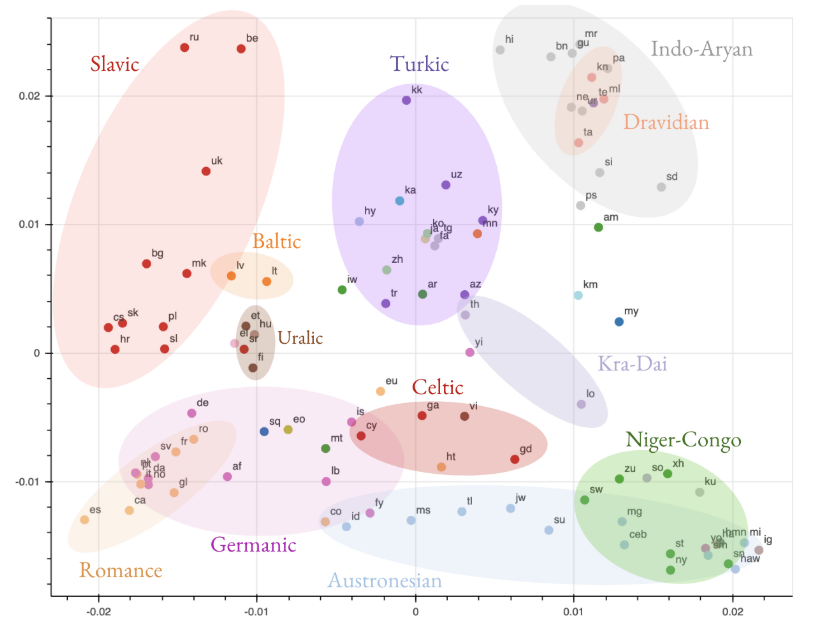
\includegraphics[width=0.6\linewidth]{./assets/relatedwork/embeddings_by_language.png}
  \caption{From \cite{kudugunta18}, visualizing clustering of the encoder representations of all languages, based on ther SVCCA similarity.}
  \label{fig:embeddings_by_language}
\end{figure}

%TODO What language model do they use? I dont see anything about BERT


\cite{lample18} uses a cyclic loss to apply unsupervised machine translation suign monolingual corpora only. 
Here, sentence-embeddings are learned over time, which follow the cyclic loss constraint, and minimize the sunsupervised translation loss.

Other work tries to disentangle the different linguisitc, visual and audio-based features by supplying multi-modal input at once \cite{ma19}.
A translation model is learned which can not only translate between different domains, but also between different modalities (i.e. from image to audio, audio to text, and any such combination).






\section{Metric Learning and Disentanglement}

\section{Zero shot and One shot learning }

\section{Clustering Algorithms}

\section{Applications of word vector}

\newpage
\subsubsection{Word2Vec}

BERT conditions on the rest of the input sentence.

BERT uses words, subwords and individual characters (in total 30'000) that are then used as tokens.

Idea is to do the following:
Concepts (and thus words), are represented across multiple contexts.
We can create probabilistic word-embeddings by sampling from a corpus the context of a specific word.
From multiple samples of the context-embedding-vector, we take the mean and stddev, or create a GMM if there are multimodal logic (we can check this multimodality by runniing some sort of rejection sampling algorithm).
Then we have a probability density function (one for each language), and can map one into another.

Perhaps we could split up too high-variance embeddings to multimodal embeddings, depending on their use-cases.

This allows for interpretability in polysemy sentences.

Not using more complex flows implies that the flow itself is not the bottleneck (they probably tried out other flows as well).

Are the individual word-embeddings going to be one big blob with high variance, or is it going to be a multi-modal distribution...?

Another task we may look at is, from a given word-embedding, sample it's context. 
Not entirely sure how to do this with BERT and co.

At what point do we overfit, and at what point do we generalize?


\textbf{Artetxe bilingual token matching through unsupervised machine translation}

- Input is cross-lignual word-embeddings
- Build an unsupervised phrase-based statistical machine translation system
- Derive phrase-based embeddings from input-word-embeddings by taking top 400'000 bigrams and 400'000 trigrams -> take arithmetic mean of word-embedding
- score top 100 close phrases using softmax cosine similarity
- generation of synthetic parallel corpus using this approach
- Then use FastAlign to use parallel corpus to align words
- 

\chapter{Analysing the current state of the art}

Upadhyay et al. argue that the choice of data is more important than the actual algorithm.

Definitely also look into this, [Analyzing the Limitations of Cross-lingual Word Embedding Mappings] seems to be an analysis of the difficulties etc. 

\section{On the Linear Separability of meaning within sampled BERT vectors}

\subsection{Motivation}

To see if there is any structure within BERT vectors w.r.t. the different meaning of one word, we ask ourselves whether or not different part of the meaning are at different locations of the embedding space produced by BERT.

\subsection{Experiment setup}

Let us regard a word $w$ in sentence $s$ is indexed by $i$.
When passed through the BERT model, the word $w$ produces an embedding $x_w$.
When we sample BERT embeddings for a single word $w$ for $n=500$ sentences. 

Let us restrict the choice of words $w$ on polysemous and ambigious words which carry multiple meanings. 
Specifically, $w$ is chosen in such a way that each meaning has more than 30 samples in each class when chosen from within the SemCor dataset. 

%TODO beautify this table

\begin{center}
% Words used to test BERT-sampled vectors for linear separability of lexical features
\begin{tabular}{ | c | c | c | }
\hline
\multicolumn{3}{ | c | }{Words used to test BERT-sampled vectors for linear separability of lexical features} \\
\hline
 was & is & be \\ 
 \hline
 are & more & one \\  
 \hline
 first & only & time \\
 \hline
\end{tabular}
\end{center}

When we sample 
Specifically, the experiment setup looks as follows.

\begin{algorithm}[H]
\SetAlgoLined
\SetKwInOut{Input}{Input}
\Input{A target word $w_{\text{target}}$; The latent dimensionality $k$for PCA;}
\KwResult{Accuracy of a logistic regression classifier}
 $\mathbf{D}, \mathbf{y} \leftarrow $  sample up to 500 sentences (as much as available) from the SemCor corpus which include the word $w_{\text{target}}$, along with the corresponding WordNet meaning-id\;

$ \mathbf{X} \leftarrow BERT( \mathbf{D} )$ i.e. pass each sentence through BERT and retrieve the resulting word embedding $x_w$ as defined in the above section\;
 
$ \mathbf{X}, \mathbf{y} \leftarrow oversample( \mathbf{X}, \mathbf{y} )$ such that we don't have dominating classes\;
 
$ \mathbf{X_\text{train}}, \mathbf{X_\text{test}}, \mathbf{y_\text{train}}, \mathbf{y_\text{test}} \leftarrow trainTestSplit( \mathbf{X}, \mathbf{y}, testProportion=0.4 )$ \;

$ \mathbf{X_\text{train}} \leftarrow StandardScaler( \mathbf{X_\text{train}})$ such that all the data is normalized\;

$ \mathbf{X_\text{train}} \leftarrow PCA( \mathbf{X_\text{train}}, k )$ such that all the data is projected to a lower latent dimensionality $k$\;

$ model \leftarrow LogisticRegression( \mathbf{X_\text{train}}, \mathbf{y_\text{train}} )$ \;
    
$ \mathbf{\hat{y}_\text{test}} \leftarrow model.predict(\mathbf{X_\text{test}})$ \;

$ accuracy, confusionMatrix \leftarrow loss(\mathbf{y_\text{test}}, \mathbf{\hat{y}_\text{test}}) $ \;
    
return $ accuracy, confusionMatrix $\;
    
 \caption{Checks sampled BERT vectors for linear interpretability by meaning}
\end{algorithm}

We use a binary 
%TODO what is the formal name of the loss function that we are using..?

First of all, we sample $n=500$ sentences from the news corpus for a target word $\hat{w}$, which has index $i$ in sentence $s$.

Each sentence, we pass through the 

The BERT model takes a sequence of size (up to) 512 elements as input.

We sample $n=500$ vectors from BERT.
This is the vector at the output embedding layer of BERT, which has the same location as the input to the BERT model.

%TODO insert graphic of which embedding is used..

We apply t-fold cross validation, and measure the mean accuracy as well as the standard deviation of the accuracy. 
We also note down the variance kept after projecting PCA on the lower dimensionality $k$.
This is the sum of the first $k$ largest normalized eigenvalues.


\subsection{Results}

The number of words we can use to realiably estimate a planar separation of semantics within the sampled BERT vectors is small.

We run the above experiment for a set of different $k$ to build up an intuition of how well different dimensionalites still capture the meaning in different locations of the vector space. 

\begin{center}
\captionof{table}{Mean and standard deviation of the accuracy of a linear classifier trained on the 2 most common classes of WordNet meanings for the word \textit{was}.}
\begin{tabular}{SSSSSSSS} \toprule
    {dimensionality} & {variance kept} & {accuracy (mean / $\pm$ stddev)}  \\ \midrule
     10  & 0.27 & 0.82 / $\pm$ 0.03 \\ \midrule
     20  & 0.41 & 0.81 / $\pm$ 0.04  \\ \midrule
     30  & 0.50 & 0.85 / $\pm$ 0.03  \\ \midrule
     50  & 0.63 & 0.92 / $\pm$ 0.03 \\ \midrule
     75  & 0.73 & 0.94 / $\pm$ 0.02 \\ \midrule
    100 & 0.81 & 0.95 / $\pm$ 0.02  \\ \midrule
\end{tabular}
\end{center}

% -> show which two different word meanings are sampled

% Also perhaps show the confusion matrix

\begin{center}
\captionof{table}{Mean and standard deviation of the accuracy of a linear classifier trained on the 2 most common classes of WordNet meanings for the word \textit{is}.}
\begin{tabular}{SSSSSSSS} \toprule
    {dimensionality} & {variance kept} & {accuracy (mean / $\pm$ stddev)}  \\ \midrule
       2  & 0.09 & 0.57 / $\pm$ 0.02 \\ \midrule
     10  & 0.29 & 0.82 / $\pm$ 0.03  \\ \midrule
     20  & 0.42 & 0.82 / $\pm$ 0.04  \\ \midrule
     30  & 0.51 & 0.83 / $\pm$ 0.03  \\ \midrule
     50  & 0.72 & 0.85 / $\pm$ 0.04 \\ \midrule
     75  & 0.78 & 0.84 / $\pm$ 0.04 \\ \midrule
    100 & 0.79 & 0.85 / $\pm$ 0.03  \\ \midrule
\end{tabular}
\end{center}

% -> show which two different word meanings are sampled

\begin{center}
\captionof{table}{Mean and standard deviation of the accuracy of a linear classifier trained on the 2 most common classes of WordNet meanings for the word \textit{one}.}
\begin{tabular}{SSSSSSSS} \toprule
    {dimensionality} & {variance kept} & {accuracy (mean / $\pm$ stddev)}  \\ \midrule
       2  & 0.10 & 0.55 / $\pm$ 0.10 \\ \midrule
       3  & 0.14 & 0.51 / $\pm$ 0.05 \\ \midrule
     10  & 0.34 & 0.59 / $\pm$ 0.08  \\ \midrule
     20  & 0.50 & 0.76 / $\pm$ 0.03  \\ \midrule
     30  & 0.62 & 0.77 / $\pm$ 0.02  \\ \midrule
     50  & 0.76 & 0.83 / $\pm$ 0.06 \\ \midrule
     75  & 0.87 & 0.87 / $\pm$ 0.05 \\ \midrule
    100 & 0.94 & 0.87 / $\pm$ 0.05  \\ \midrule
\end{tabular}
\end{center}

There are many permutations 
We now also employ multi-class classificiation.

\begin{center}
\captionof{table}{Mean and standard deviation of the accuracy of a linear classifier trained on the the 4 most common classes of WordNet meanings for the word \textit{was}.}
\begin{tabular}{SSSSSSSS} \toprule
    {dimensionality} & {variance kept} & {accuracy (mean / $\pm$ stddev)}  \\ \midrule
       2  & 0.08 & 0.38 / $\pm$ 0.03 \\ \midrule
       3  & 0.11 & 0.38 / $\pm$ 0.04 \\ \midrule
     10  & 0.28 & 0.65 / $\pm$ 0.03  \\ \midrule
     20  & 0.43 & 0.76 / $\pm$ 0.04  \\ \midrule
     30  & 0.53 & 0.83 / $\pm$ 0.03  \\ \midrule
     50  & 0.67 & 0.93 / $\pm$ 0.01 \\ \midrule
     75  & 0.77 & 0.95 / $\pm$ 0.01 \\ \midrule
    100 & 0.83 & 0.95 / $\pm$ 0.01  \\ \midrule
\end{tabular}
\end{center}

We get very similar accuracies for "time", "made", "thought".
However, these tables are left out as we do not deem these to be statistically significant.

%TODO re-run these experiments and print out the respective ids

%TODO Inseert confusion matrix here maybe




\section{On the Clusterability of meaning within sampled BERT vectors}

\subsection{Motivation}

%TODO Talk about different ways to determine if a dataset is clusteerable, but mention that in the end we want a practical approach, thus we brute-force search
%TODO 

\subsection{Experiment setup}

The general algorithm to cluster the dataset is shown below.

%TODO include optimization loop over all models

%TODO Define and show what the random adjusted index is

\begin{algorithm}[H]
\SetAlgoLined
\SetKwInOut{Input}{Input}
\Input{
$w_{\text{target}}$: The target word whose BERT vectors we want to cluster; \\ 
$DimRed$: The dimensionality reduction method; \\
$k$ : The latent dimensionality for the dimensionality reduction method; \\ 
$ClusterAlgorithm$: The clustering algorithm to use;
%TODO insert optional l1/l2 normalization
}
\KwResult{The associated cluster-id with each sampled sentence, and the adjusted random index.}

 $\mathbf{D}, \mathbf{y} \leftarrow $  sample up to 500 sentences from the SemCor corpus which include the word $w_{\text{target}}$, along with the corresponding WordNet meaning-id, and compensate more sentences by sampling from the news corpus if less than 500 sentences are available in the SemCor sentence.
We set y = -1 whenever no labeling information is available, which is the case if we don't sample data from the SemCor corpus.\;

$ \mathbf{X} \leftarrow BERT( \mathbf{D} )$ i.e. pass each sentence through BERT and retrieve the resulting word embedding $x_w$ as defined in the above section\;
 
$ \mathbf{X}, \mathbf{y} \leftarrow oversample( \mathbf{X}, \mathbf{y} )$ such that we don't have dominating classes (all except for $y = -1$).\;
 
$ \mathbf{X} \leftarrow StandardScaler( \mathbf{X})$ such that all the data is normalized\;

$ \mathbf{X} \leftarrow DimRed( \mathbf{X}, k )$ such that all the data is projected to a lower latent dimensionality $k$\;

$ model \leftarrow ClusterAlgorithm( \mathbf{X})$ \;

$ \mathbf{\hat{y}} \leftarrow model.predict(\mathbf{X}) $ \;

$ score \leftarrow AdjustedRandomIndex(\mathbf{\hat{y}}, \mathbf{y}) $ \;

return $ score, \mathbf{\hat{y}}$\;
    
 \caption{Checks sampled BERT vectors for clusters by  meaning}
\end{algorithm}

However, because some simple algor.

We had a few constraints.
When clustering, we are not given the number of cluster to be found. 
Thus, the algorithm must solve the multi-modal detection problem intrinsically, which is considered a hard problem in machine learning, as it falls in the same category as global probability density estimation.
Also, because we use the lexical distinction of semantics as defined in WordNet, our algorithm needs to adapt to the granularity that was defined by linguists.

Because we want to evaluate how well our clustering method can mimick the semantic definitions in WordNet, but also generalize to unseen words, we train on an unsupervised dataset. 
We then test our resulting clustering on a labeled datasetet using the random adjusted index \cite{rand71}, \cite{hubert85}.

The adjusted random index calculates the overlap and as such the similarity between two clustering assignments.
Specifically, 

\begin{equation}
A R I=\frac{\sum_{i j}\left(^{n_{i j}}\right)-\left[\sum_{i}\left(\begin{array}{c}a_{i} \\ 2\end{array}\right) \sum_{j}\left( \begin{array}{c}b_{j} \\ 2\end{array} \right)\right] /\left(\begin{array}{c}n \\ 2\end{array}\right)}{\frac{1}{2}\left[\sum_{i}\left(\begin{array}{c}a_{i} \\ _{2}\end{array}\right)+\sum_{j}\left(\begin{array}{l}b_{j} \\ 2\end{array}\right)\right]-\left[\sum_{i}\left(\begin{array}{c} a_{i} \\ 2\end{array}\right) \sum_{j}\left(\begin{array}{l}b_{j} \\ 2\end{array}\right)\right] /\left(\begin{array}{l}n \\ 2\end{array}\right)}
\end{equation}{\label{eq:adjustedrandomindex}}

%TODO read this up again!
where $n_{i,j}$ is the number of items that are present in both clustering assignment, $a_i = \sum_j n_{i,j}$ , $b_j = \sum_i n_{i,j}$ for two clustering $a$ and $b$.

where the resulting score is between $[-1.0, 1.0]$, where a score of $0$ implies completely assignment of cluster-labels into random buckets, $-1.0$ implies a negative correlation, and $1.0$ implies perfect similarity.
The adjusted random index is adjusted for chance, by taking all possible permutations of the labels that the clustering algorithm can have.




Although we will not go into too much detail with the algorithm descriptions here, we will 


The general algorithm to cluster the dataset is shown below.



\begin{enumerate}
\item s
\end{enumerate}

%TODO talk about the chinese whispers algorithm bcs this is custom-made

\subsection{Results}

%\begin{center}
%\captionof{table}{Adjusted Random Index between the predicted cluster labels and the true underlying cluster labels. 
%Cluster labels correspond to the different meanings in WordNet.
%BERT vectors are sampled for the word "use". 
%We sample 500 vectors and project these to 50 dimensions before clustering.
%}
%\begin{tabular}{SSSSSSSS} \toprule
%    {model} & {best adjusted random score} & {best adjusted random score)}  \\ \midrule
%       Affinity Propagation  & 0.001 & 0.38 / $\pm$ 0.03 \\ \midrule
%       DBScan                     & 0.000 & 0.38 / $\pm$ 0.04 \\ \midrule
%      HDBScan                    & 0.328 & 0.65 / $\pm$ 0.03  \\ \midrule
%     MeanShift                   & 0.004 & 0.76 / $\pm$ 0.04  \\ \midrule
%     Optics                        & 0.000 & 0.83 / $\pm$ 0.03  \\ \midrule
%\end{tabular}
%\end{center}

\newcolumntype{b}{X}
\newcolumntype{s}{>{\hsize=.5\hsize}X}

\begin{table}[htbp]
    \centering
    %\begin{tabularx}{\textwidth}{| X | X |}
    \begin{tabularx}{\textwidth}{b|ss}
    \toprule
      {model} & {ARI)}  \\ \hline
        Affinity Propagation     & 0.001     \\ \hline
        DBScan                        & 0.000      \\ \hline
        HDBScan                      & 0.328     \\ \hline
        MeanShift                    & 0.004      \\ \hline
        Optics                         & 0.000      \\ \hline
    \end{tabularx}
\end{table}

Repeating the experiment with 1000 datapoint does not change the results by much.

\begin{table}[htbp]
    \centering
    %\begin{tabularx}{\textwidth}{| X | X |}
    \begin{tabularx}{\textwidth}{b|ss}
    \toprule
      {model} & {ARI)}  \\ \hline
        Affinity Propagation     & 0.000     \\ \hline
        DBScan                        & 0.139      \\ \hline
        HDBScan                      & 0.271     \\ \hline
        MeanShift                    & 0.005      \\ \hline
        Optics                         & 0.070      \\ \hline
    \end{tabularx}
\end{table}

Repeating the experiment with 1000 items and projecting PCA to 100 results in 

\begin{table}[htbp]
    \centering
    %\begin{tabularx}{\textwidth}{| X | X |}
    \begin{tabularx}{\textwidth}{b|ss}
    \toprule
      {model} & {ARI)}  \\ \hline
        Affinity Propagation     & 0.000     \\ \hline
        DBScan                        & 0.215      \\ \hline
        HDBScan                      & 0.359     \\ \hline
        MeanShift                    & 0.003      \\ \hline
        Optics                         & 0.000      \\ \hline
    \end{tabularx}
\end{table}

We see that including more dimensions make the clustering better w.r.t. the adjusted random score.

%TODO Move to 
Here, we also introduce the chinese whispers algorithm.
The chinese whispers algorithm was used to cluster for word-senses in the context of static word embeddings, such as in
\cite{pelevina16}.

We now apply forceful clustering using Bayesian Optimization.

%TODO: Move some to Appendix (especially when it is not very successful...
100 latent dimensions, 500 samples
\begin{table}[htbp]
    \centering
    %\begin{tabularx}{\textwidth}{| X | X |}
    \begin{tabularx}{\textwidth}{b|ss}
    \toprule
      {model} & {ARI)}  \\ \hline
        Affinity Propagation     & 0.168     \\ \hline
        Chinese Whispers        & 0.298     \\ \hline
        DBScan                        & 0.201      \\ \hline
        HDBScan                      & 0.242     \\ \hline
        MeanShift                    & 0.167      \\ \hline
        Optics                         & 0.167      \\ \hline
    \end{tabularx}
\end{table}


100 components, 1000 samples
\begin{table}[htbp]
    \centering
    %\begin{tabularx}{\textwidth}{| X | X |}
    \begin{tabularx}{\textwidth}{b|ss}
    \toprule
      {model} & {ARI)}  \\ \hline
        Affinity Propagation     & 0.170     \\ \hline
        Chinese Whispers        & 0.249     \\ \hline
        DBScan                        & 0.260      \\ \hline
        HDBScan                      & 0.234     \\ \hline
        MeanShift                    & 0.167      \\ \hline
        Optics                         & 0.197      \\ \hline
    \end{tabularx}
\end{table}


Projecting to lower dimensions increases accuracy strongly.
20 components, 1000 samples
\begin{table}[htbp]
    \centering
    %\begin{tabularx}{\textwidth}{| X | X |}
    \begin{tabularx}{\textwidth}{b|ss}
    \toprule
      {model} & {ARI)}  \\ \hline
        Affinity Propagation     & 0.165     \\ \hline
        Chinese Whispers        & 0.349     \\ \hline
        DBScan                        & 0.167      \\ \hline
        HDBScan                      & 0.273     \\ \hline
        MeanShift                    & 0.226      \\ \hline
        Optics                         & 0.167      \\ \hline
    \end{tabularx}
\end{table}



Projecting to lower dimensions increases accuracy strongly.
and now we add a SEP token
20 components, 1000 samples
\begin{table}[htbp]
    \centering
    %\begin{tabularx}{\textwidth}{| X | X |}
    \begin{tabularx}{\textwidth}{b|ss}
    \toprule
      {model} & {ARI}  \\ \hline
        Affinity Propagation     & 0.316     \\ \hline
        Chinese Whispers        & 0.457     \\ \hline
        DBScan                        & 0.170      \\ \hline
        HDBScan                      & 0.298     \\ \hline
        MeanShift                    & 0.251      \\ \hline
        Optics                         & 0.167      \\ \hline
    \end{tabularx}
\end{table}

We now analyse the embeddings manually

\begin{figure}
\begin{subfigure}{.5\textwidth}
  \centering
  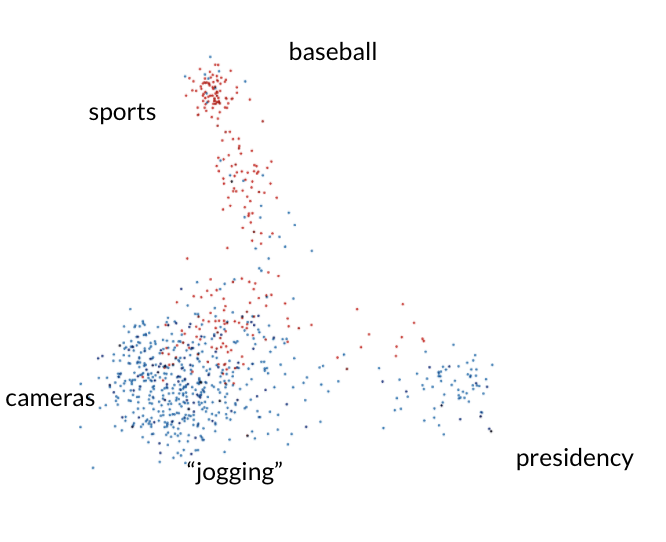
\includegraphics[width=.8\linewidth]{./assets/analysis/run_pca.png}
  \caption{1a}
  \label{fig:sfig1}
\end{subfigure}%
\begin{subfigure}{.5\textwidth}
  \centering
  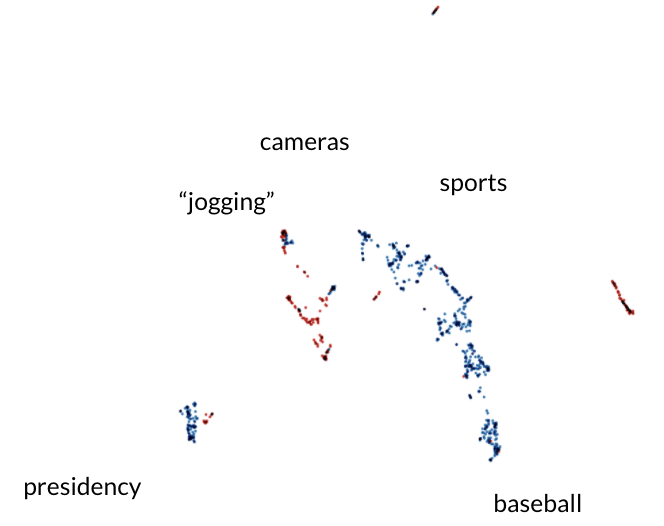
\includegraphics[width=.8\linewidth]{./assets/analysis/run_umap.png}
  \caption{1b}
  \label{fig:sfig2}
\end{subfigure}
\caption{plots of....}
\label{fig:fig}
\end{figure}



\begin{figure}
\begin{subfigure}{.5\textwidth}
  \centering
  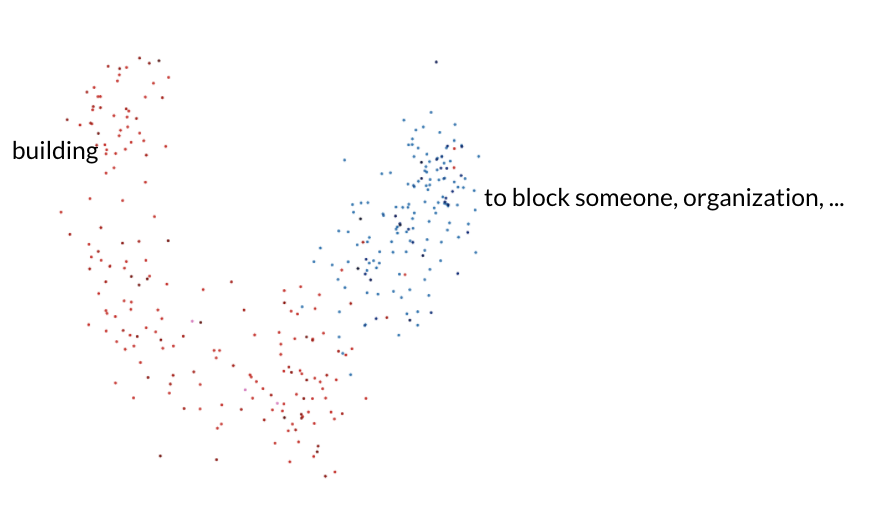
\includegraphics[width=.8\linewidth]{./assets/analysis/block_pca.png}
  \caption{1a}
  \label{fig:sfig1}
\end{subfigure}%
\begin{subfigure}{.5\textwidth}
  \centering
  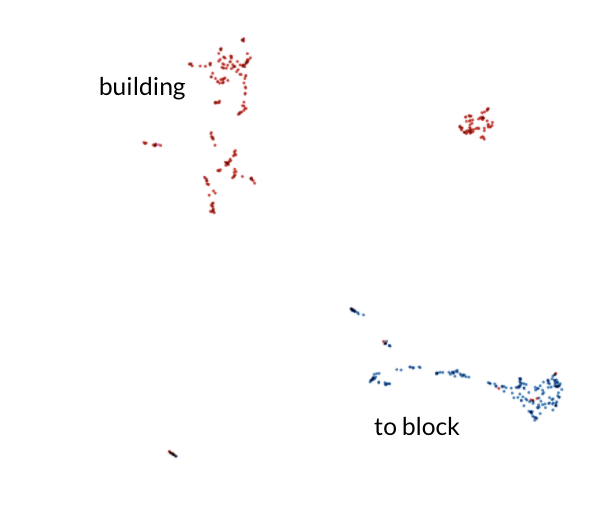
\includegraphics[width=.8\linewidth]{./assets/analysis/block_umap.png}
  \caption{1b}
  \label{fig:sfig2}
\end{subfigure}
\caption{plots of....}
\label{fig:fig}
\end{figure}



\begin{figure}
\begin{subfigure}{.5\textwidth}
  \centering
  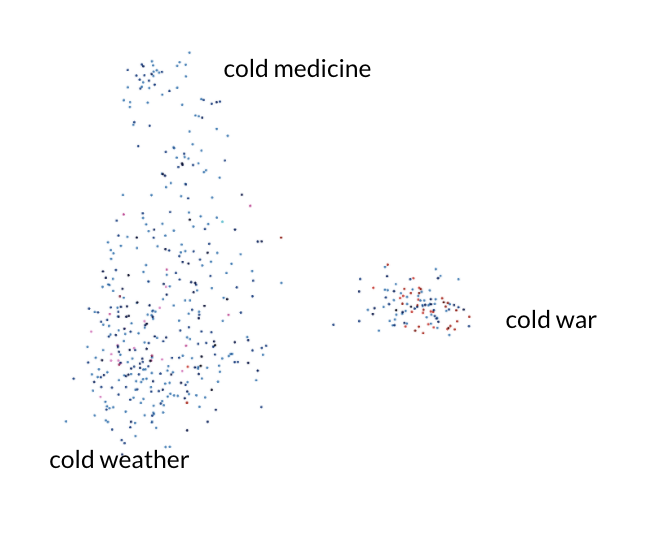
\includegraphics[width=.8\linewidth]{./assets/analysis/cold_pca.png}
  \caption{1a}
  \label{fig:sfig1}
\end{subfigure}%
\begin{subfigure}{.5\textwidth}
  \centering
  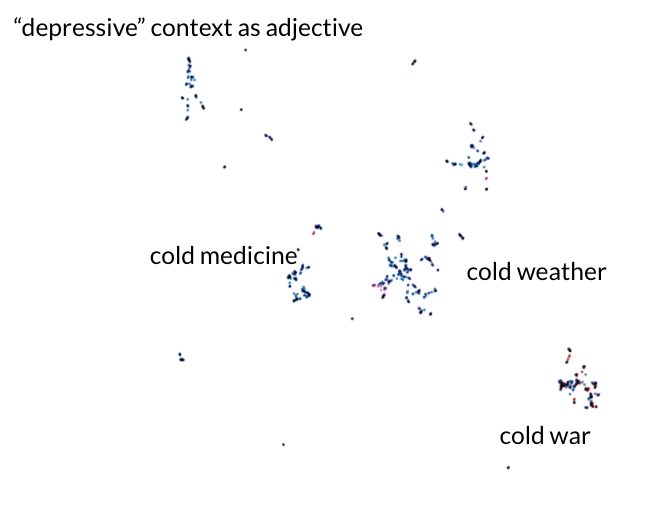
\includegraphics[width=.8\linewidth]{./assets/analysis/cold_umap.png}
  \caption{1b}
  \label{fig:sfig2}
\end{subfigure}
\caption{plots of....}
\label{fig:fig}
\end{figure}

\subsubsection{Qualitative evaluation}

Given that the above numbers likely don't mean anything, here are some clusters found for the best model configuration (chinese whispers), applied on a set of words.



Can see that this can be used for biased and insecure AI applications!

\begin{figure}[H]
\begin{align}
\text{                                                                  } & \text{- - - -} \nonumber \\
\text{Ms. Gotbaum tried to slide her handcuffed } & \text{arms from her back to her front} \nonumber \\
\text{                                                                  } & \text{- - - -} \nonumber \\
               \text{That magisterial use of the upper body and } & \text{arms is her physical signature} \nonumber \\
\text{entered the stage in pairs and forcefully stretched their } & \text{arms and legs} \nonumber \\ 
                                    \text{ripped from patients’ } & \text{arms as they were carried away} \nonumber \\
                                    \text{                                                                  } & \text{- - - -} \nonumber \\
\end{align}
\caption{A famous equation}
\end{figure}


\begin{figure}[H]
\begin{align}
\text{                                              } & \text{- - - -} \nonumber \\
\text{She swooped him up into her } & \text{arms and kissed him madly} \nonumber \\
\text{                                              } & \text{- - - -} \nonumber \\
\text{I place my son in her } & \text{arms and I pray that it somehow comforts her} \nonumber \\
\text{perfect babies \ldots into the loving } & \text{arms of middle class+ Americans} \nonumber \\
\text{which he falls back into her } & \text{arms like a baby} \nonumber \\
\text{Sometimes I took it into my } & \text{arms and felt its surprising heft} \nonumber \\
\text{                                              } & \text{- - - -} \nonumber
\end{align}
\caption{A famous equation}
\end{figure}


\begin{figure}[H]
\begin{align}
\text{                              } & \text{- - - -} \nonumber \\
\text{and shuttle robotic } & \text{arms of a solar array and truss}  \nonumber\\
\text{                              } & \text{- - - -} \nonumber \\
\text{a contingent of young } & \text{arms that will allow us to win now}  \nonumber\\
\text{By and large, those } & \text{arms remained as fictional as those in "The War \ldots"}  \nonumber\\
\text{and extensive use of robotic } & \text{arms operating at their limits}  \nonumber\\
\text{staff of strong young } & \text{arms that might have tamed the National League East} \nonumber \\
\text{                              } & \text{- - - -} \nonumber \\
\end{align}
\caption{A famous equation}
\end{figure}



\begin{figure}[H]
\begin{align}
\text{                                                   } & \text{- - - -} \nonumber \\
\text{this country is so polarized that people spring to } & \text{arms against any proposal} \nonumber \\
\text{                                                   } & \text{- - - -} \nonumber \\
                        \text{At least they are carrying } & \text{arms to protect themselves} \nonumber \\
                 \text{His organization issued a call to } & \text{arms} \nonumber \\
      \text{he shoves it in the faces of his comrades in } & \text{arms} \nonumber \\
                           \text{people who had taken up } & \text{arms against the United States} \nonumber \\
                    \text{Mostly non-Arab rebels took up } & \text{arms in early 2003} \nonumber \\
\text{                                                   } & \text{- - - -} \nonumber \\
\end{align}
\caption{A famous equation}
\end{figure}


\begin{figure}[H]
\begin{align}
\text{                                                   } & \text{- - - -} \nonumber \\
                      \text{The classic years of the} & \text{arms race, the 1950s and ’60s before} \nonumber \\
                      \text{                                                   } & \text{- - - -} \nonumber \\
                    \text{that concerns over nuclear} & \text{arms proliferation in the Middle East} \nonumber \\
                  \text{Russian adherence to another} & \text{arms control treaty} \nonumber \\
       \text{he will press for peace and an eventual} & \text{arms cut for the states} \nonumber \\
       \text{payments to the companies that supplied} & \text{arms to Iraq were often delayed} \nonumber \\
\text{Mr. Safar denies any wrongdoing, including any} & \text{arms dealings} \nonumber \\
\text{                                                   } & \text{- - - -} \nonumber \\
\end{align}
\caption{A famous equation}
\end{figure}



\begin{figure}[H]
\begin{align}
\text{                                              } & \text{- - - -} \nonumber \\
           \text{leaned back in his chair and, with} & \text{ arms crossed,} \nonumber \\
\text{                                              } & \text{- - - -} \nonumber \\
\text{God, fully in name, is at the bottom with his} & \text{ arms out wide.} \nonumber \\
    \text{If you feel yourself falling, spread your} & \text{ arms} \nonumber \\
                                   \text{Agamemnon,} & \text{ arms raised ... barely contained violence} \nonumber \\
                       \text{Mr. James sat with his} & \text{ arms folded, his head lowered} \nonumber \\
      \text{she felt tears in her eyes and held her} & \text{ arms out in simple joy} \nonumber \\
\text{                                             } & \text{- - - -} \nonumber \\
\end{align}
\caption{A famous equation}
\end{figure}

NOW MOVING OVER TO THE BANK EXAMPLE


\begin{figure}[H]
\begin{align}
\text{                                                 } & \text{- - - -} \nonumber \\
\text{heavy withdrawals from the British} & \text{ bank Northern Rock reignited concern} \nonumber \\
\text{                                                 } & \text{- - - -} \nonumber \\
\text{credit card and other consumer loans, forcing the} & \text{ bank to set aside \$3.4 billion} \nonumber \\
\text{by a mainland Chinese commercial bank in a U.S.} & \text{ bank} \nonumber \\
\text{Investors fear the} & \text{ bank will be forced to write down} \nonumber \\
\text{investors hoped that the} & \text{ bank had disclosed the} \nonumber \\
\text{                                                 } & \text{- - - -} \nonumber \\
\end{align}
\caption{A famous equation}
\end{figure}


\begin{figure}[H]
\begin{align}
\text{                                              } & \text{- - - -} \nonumber \\
\text{I would expect the} & \text{ bank by the trail to the left of the road to have been broken down} \nonumber \\
\text{                                              } & \text{- - - -} \nonumber \\
\text{The current slowed and swirled alongside a mud} & \text{ bank where cows had trodden to the water} \nonumber \\
\text{But the} & \text{ bank had positioned itself well} \nonumber \\
\text{provide plant scientists and farmers with a} & \text{ bank of genes} \nonumber \\
\text{Upstairs at the large} & \text{ bank of cashiers} \nonumber \\
\text{                                              } & \text{- - - -} \nonumber \\
\end{align}
\caption{A famous equation}
\end{figure}


\begin{figure}[H]
\begin{align}
\text{                                                 } & \text{- - - -} \nonumber \\
\text{of their family’s naturalization —} & \text{ bank deposit by bank deposit} \nonumber \\
\text{                                                 } & \text{- - - -} \nonumber \\
\text{12 that the company might suffer a run on the} & \text{ bank because of mortgage concerns} \nonumber \\
\text{Third, per several} & \text{ bank managers of major national banks} \nonumber \\
\text{Local party bosses gained broad powers over state} & \text{ bank lending, taxes} \nonumber \\
\text{government contracts, and a web of} & \text{ bank accounts} \nonumber \\
\text{Prince Bandar’s Washington} & \text{ bank accounts} \nonumber \\
\text{                                                 } & \text{- - - -} \nonumber \\
\end{align}
\caption{A famous equation}
\end{figure}


\begin{figure}[H]
\begin{align}
\text{                                                    } & \text{- - - -} \nonumber \\
 \text{to lift some of the mystery surrounding the central} & \text{ bank and improve communications with Wall Street} \nonumber \\
\text{                                                    } & \text{- - - -} \nonumber \\
\text{many economists had predicted that the} & \text{ bank would not cut its rate} \nonumber \\
\text{expectations that the central} & \text{ bank will raise interest} \nonumber \\
\text{a hint that the central} & \text{ bank plans to hold rates} \nonumber \\
\text{China’s central} & \text{ bank has stepped up its already huge purchases of dollar-denominated securities} \nonumber \\
\text{fertilizer prices in African countries, but that the} & \text{ bank itself had often failed to recognize} \nonumber \\
\text{                                                    } & \text{- - - -} \nonumber \\
\end{align}
\caption{A famous equation}
\end{figure}


\begin{figure}[H]
\begin{align}
\text{                                              } & \text{- - - -} \nonumber \\
\text{citing challenges for the investment} & \text{ bank and the potential for an above-average credit burden} \nonumber \\
\text{                                              } & \text{- - - -} \nonumber \\
\text{93 percent drop in profits at its investment} & \text{ bank last week} \nonumber \\
\text{UBS said it did not expect its investment} & \text{ bank to return to profitability} \nonumber \\
\text{defrauded by the investment} & \text{ bank in 1998 when} \nonumber \\
\text{said in an interview that the investment} & \text{ bank approached him last month \nonumber} \\
\text{said the leaders of Citigroup’s investment} & \text{ bank and alternative} \nonumber \\
\text{                                            } & \text{- - - -} \nonumber \\
\end{align}
\caption{A famous equation}
\end{figure}

EXAMPLES FOR KEY CLUSTERING

\begin{figure}[H]
\begin{align}
\text{                                                 } & \text{- - - -} \nonumber \\
\text{Many of the} & \text{ key Arab states } \nonumber \\
\text{                                                 } & \text{- - - -} \nonumber \\
\text{in two months and Australia's} & \text{ key S\&P ASX 200 shed 1.9 percent } \nonumber \\
\text{Wall Street rebounded Wednesday after} & \text{ key earnings reports from JPMorgan Chase \& Co.} \nonumber \\
\text{The Democratic candidate hires a} & \text{ key strategist} \nonumber \\
\text{[CLS] Mr. Jones “quickly established a good rapport with} & \text{ key donors” } \nonumber \\
\text{able to meet the two} & \text{ key officials in the government} \nonumber \\
\text{                                                 } & \text{- - - -} \nonumber \\
\end{align}
\caption{A famous equation}
\end{figure}



\begin{figure}[H]
\begin{align}
\text{                                                 } & \text{- - - -} \nonumber \\
\text{former president of Trinity College, who played a} & \text{ key role in designing the test} \nonumber \\
\text{                                                 } & \text{- - - -} \nonumber \\
\text{seen in the West as a} & \text{ key yardstick of the fairness of an election} \nonumber \\
\text{treat ... as a} & \text{ key factor in its decisions about regulatory issues} \nonumber \\
\text{which policy makers have called the} & \text{ key test for deciding whether to lower interest rates} \nonumber \\
\text{9. 11. as a} & \text{ key element in pitch meetings} \nonumber \\
\text{                                                 } & \text{- - - -} \nonumber \\
\end{align}
\caption{A famous equation}
\end{figure}



\begin{figure}[H]
\begin{align}
\text{                                                 } & \text{- - - -} \nonumber \\
\text{Interstate 5 is a} & \text{ key route connecting Southern and Northern California} \nonumber \\
\text{                                                 } & \text{- - - -} \nonumber \\
\text{ A} & \text{ key piece of new functionality for Ops Center } \nonumber \\
\text{Youssef Squali at Jefferies \& Co. says two} & \text{ key factors are driving the stock up} \nonumber \\
\text{transforming connection with believers is a} & \text{ key element of evangelical Christianity} \nonumber \\
\text{What would you say was the} & \text{ key element of your management style that allowed you to stabilize H.P.} \nonumber \\
\text{is a} & \text{ key indicator of retailer performance} \nonumber \\
\text{in the West the} & \text{ key players were not a small group of intellectuals reading Greek sources } \nonumber \\
\text{                                                 } & \text{- - - -} \nonumber \\
\end{align}
\caption{A famous equation}
\end{figure}

\begin{figure}[H]
\begin{align}
 \text{                                                 } & \text{- - - -} \nonumber \\
\text{times change and technology advances, the} & \text{ key to the city symbolizes } \nonumber \\
\text{                                                 } & \text{- - - -} \nonumber \\
\text{And an official, five-and-three-quarters-inch-long gold-plated pewter} & \text{ key to prove it} \nonumber \\
\text{but it is small enough to fit onto a} & \text{ key chain} \nonumber \\
\text{In it lay three keys on a} & \text{ key chain in the shape of a red speedboat} \nonumber \\
\text{                                                 } & \text{- - - -} \nonumber \\
\end{align}
\caption{A famous equation}
\end{figure}


\begin{figure}[H]
\begin{align}
\text{                                                 } & \text{- - - -} \nonumber \\
\text{The Red Sox will now have all their} & \text{ key players from their 2007 championship team} \nonumber \\
\text{                                                 } & \text{- - - -} \nonumber \\
\text{Mike Green scored 12 points and had a} & \text{ key assist in overtime as No. 22 Butler beat Virginia Tech} \nonumber \\
\text{or taking the chance of losing a} & \text{ key player to injury} \nonumber \\
\text{But they never led, could not get a} & \text{ key basket at crucial times and played like a team } \nonumber \\
  \text{but Cam Long stole the ball near the top of the} & \text{ key and ran out the clock} \nonumber \\
\text{                                                 } & \text{- - - -} \nonumber \\
\end{align}
\caption{A famous equation}
\end{figure}


\begin{figure}[H]
\begin{align}
\text{                                                 } & \text{- - - -} \nonumber \\
\text{Three of their} & \text{ key players played more than 40 minutes in Sacramento} \nonumber \\
\text{                                                 } & \text{- - - -} \nonumber \\
\text{A} & \text{ key for the Giants on Sunday} \nonumber \\
\text{chemical reactions on solid surfaces, which are} & \text{ key to understanding questions like why the ozone layer is thinning} \nonumber \\
\text{but is she part of the conspiracy or the} & \text{ key to Sim’s salvation?} \nonumber \\
\text{whose ability to play on a sprained ankle against the Eagles} & \text{ key to that matchup} \nonumber \\
\text{Horses have been the lifelong} & \text{ key to satisfying the real feminine needs for me and my daughter} \nonumber \\
\text{Connecticut cornerback said the} & \text{ key to defeating Louisville would be pressuring Brohm} \nonumber \\
\text{                                                 } & \text{- - - -} \nonumber \\
\end{align}
\caption{A famous equation}
\end{figure}






\section{Correlation between Part of Speech and Context within BERT}

\subsection{Motivation}

%TODO think about why you did this lol
Because there are more resources in NLP with Part of Speech (PoS) tags, as compared to semantics, we want to analyse to what extent BERT sees similarities between PoS and, and because we assume a strong correlation between PoS and semantics, we analyse to what extent this is visible within BERT vectors.

\subsection{Experiment setup}

We test the hypothesis "semantics implies PoS" by conductin the following experiment.
For a chosen target word $w_t$, we fixate one of the wordnet meanings.
We then sample $n$ sentences for the target word $w_t$ where $w_t$ has semantic meaning $m$ in the occurring sentence.
After we have sampled all the sentences, we determine the PoS for the target word $w_t$.
We then calculate the percentage occurrence of the majority PoS class and record this as a percentage.
If all of the sampled target words $w_t$ for all the sentences have the same assigned PoS tag, then the score results in a value of $1.0$.
If the dominant PoS tag occurs only half the time, this number decreases to $0.5$.
Please notice that in this experiment, we only view simple PoS tags (i.e. "noun", "verb", "adjective", "pronoun"), and not the more complex ones listed above.

%TODO perhaps give an example
%TODO explain again

\subsection{Results}

It is apparent that there is a strong relation between PoS and meaning. 
Especially "erstarrte" Verben are a strong part of this


%TODO make another plot which is more coarse

%\chapter{Evaluation} 
\chapter{Our Method}

We introduce \textit{split-words}, for which we will be generating more detailed embeddings.
The idea behind this is that introducing more specialized embeddings for certain tokens will allow to model more complex distributions.

Because the non-modified (vanilla) BERT model uses a certain workflow, we will shortly introduce BERTs pipeline.

\begin{figure}[h]
	\center
  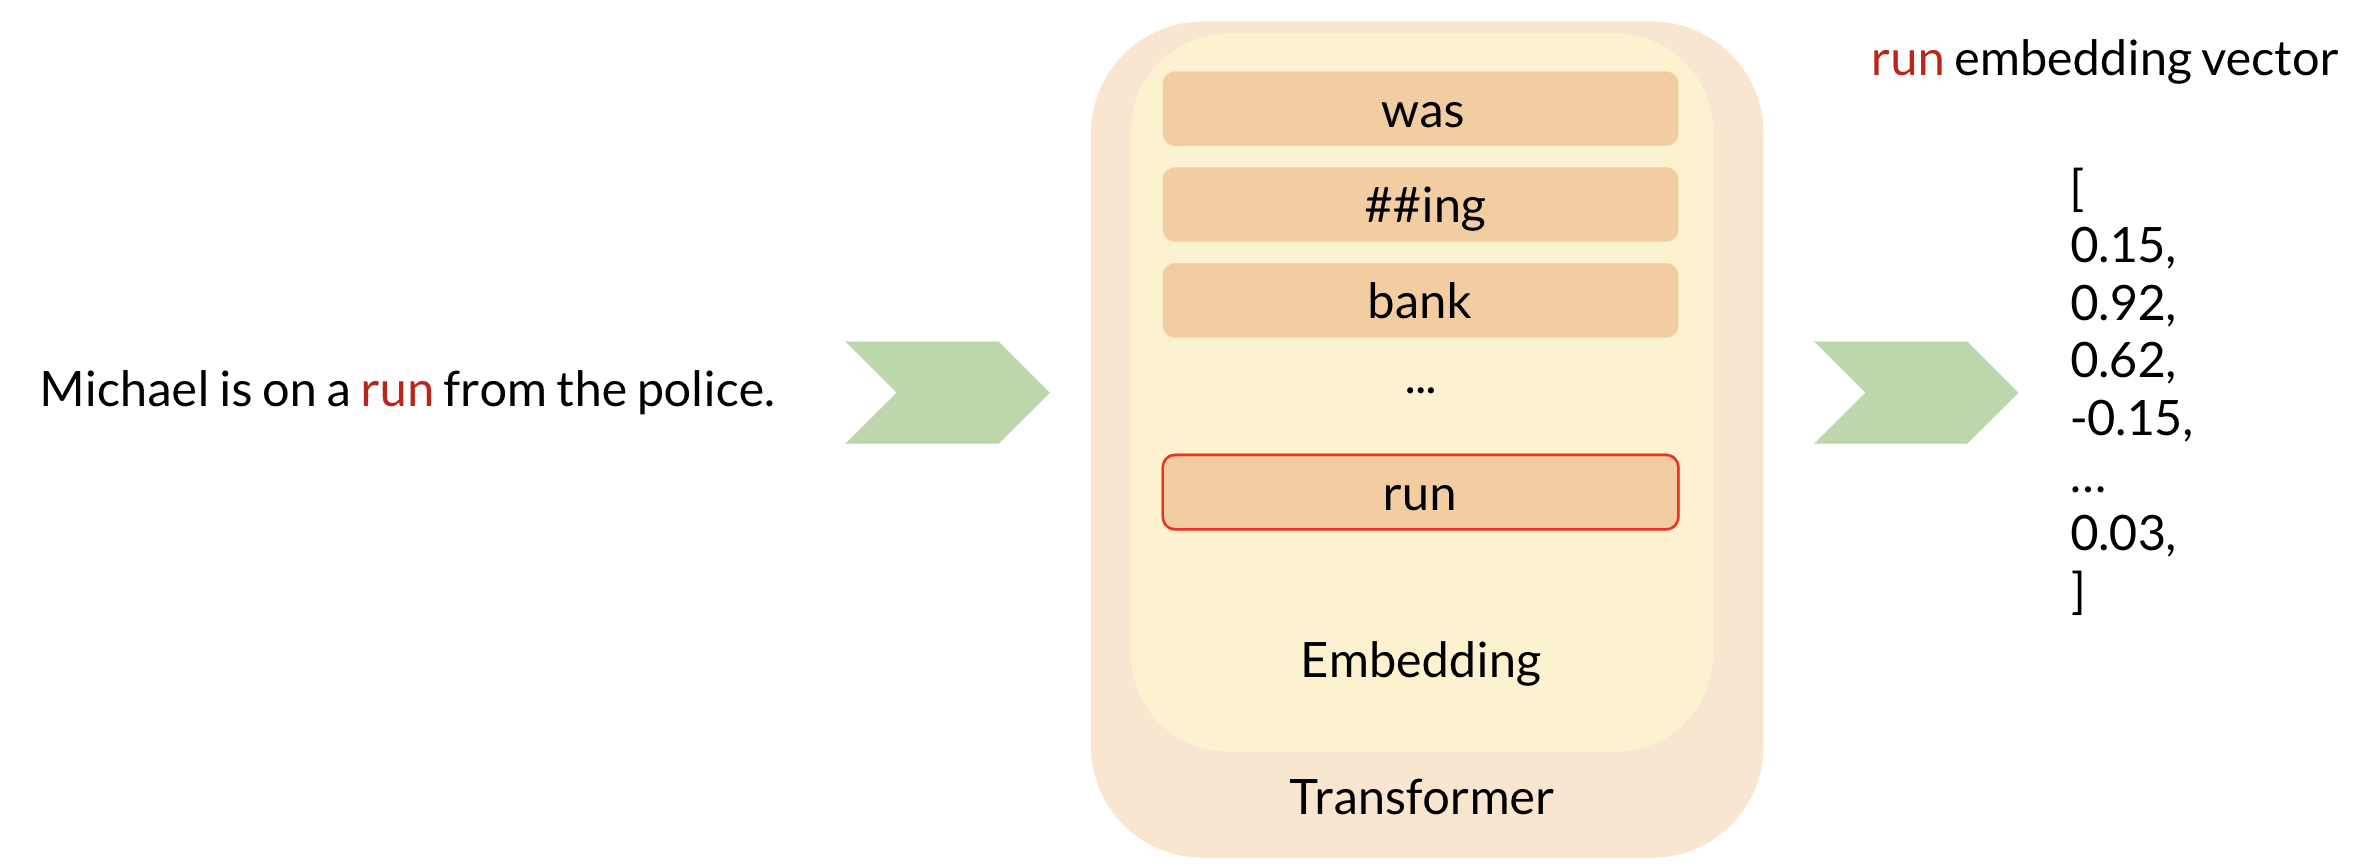
\includegraphics[width=\linewidth]{./assets/experiments/pipeline_vanilla_BERT.png}
  \caption{}
  \label{fig:cbow_skipgram}
\end{figure}


\subsection{BERnie PoS}

\subsubsection{Motivation}

\subsubsection{Experiment setup}

BERnie PoS introduces one new embedding vector for each possible PoS configuration of the split-words.

\begin{figure}[h]
	\center
  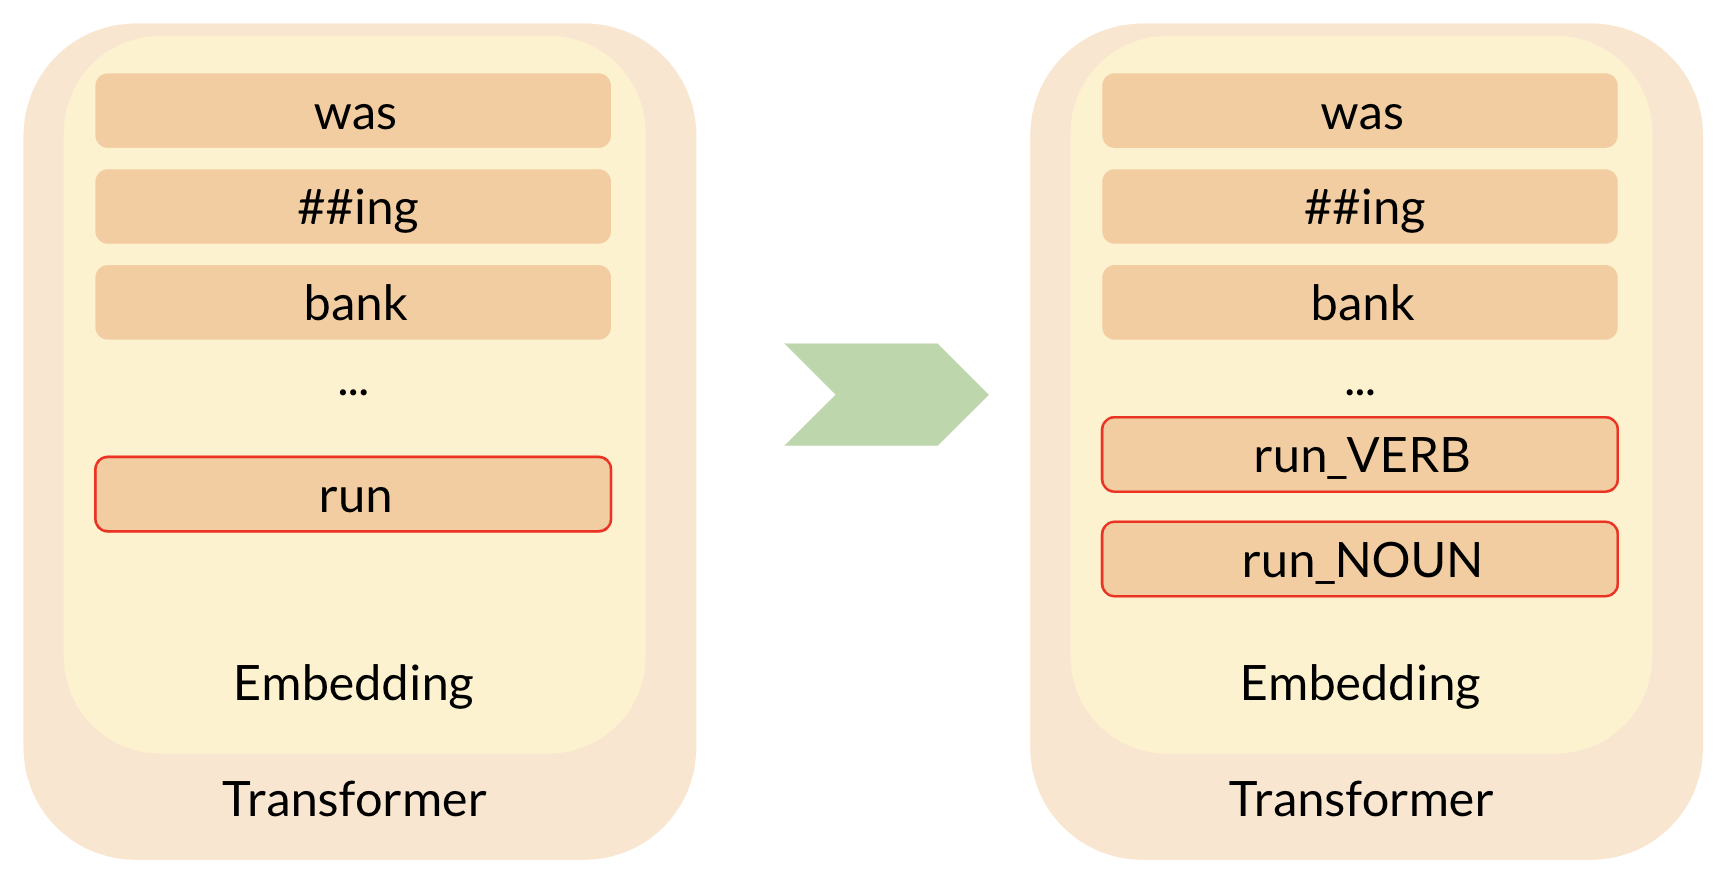
\includegraphics[width=\linewidth]{./assets/experiments/pipeline_model_BERnie_POS.png}
  \caption{}
  \label{fig:cbow_skipgram}
\end{figure}

\begin{figure}[h]
	\center
  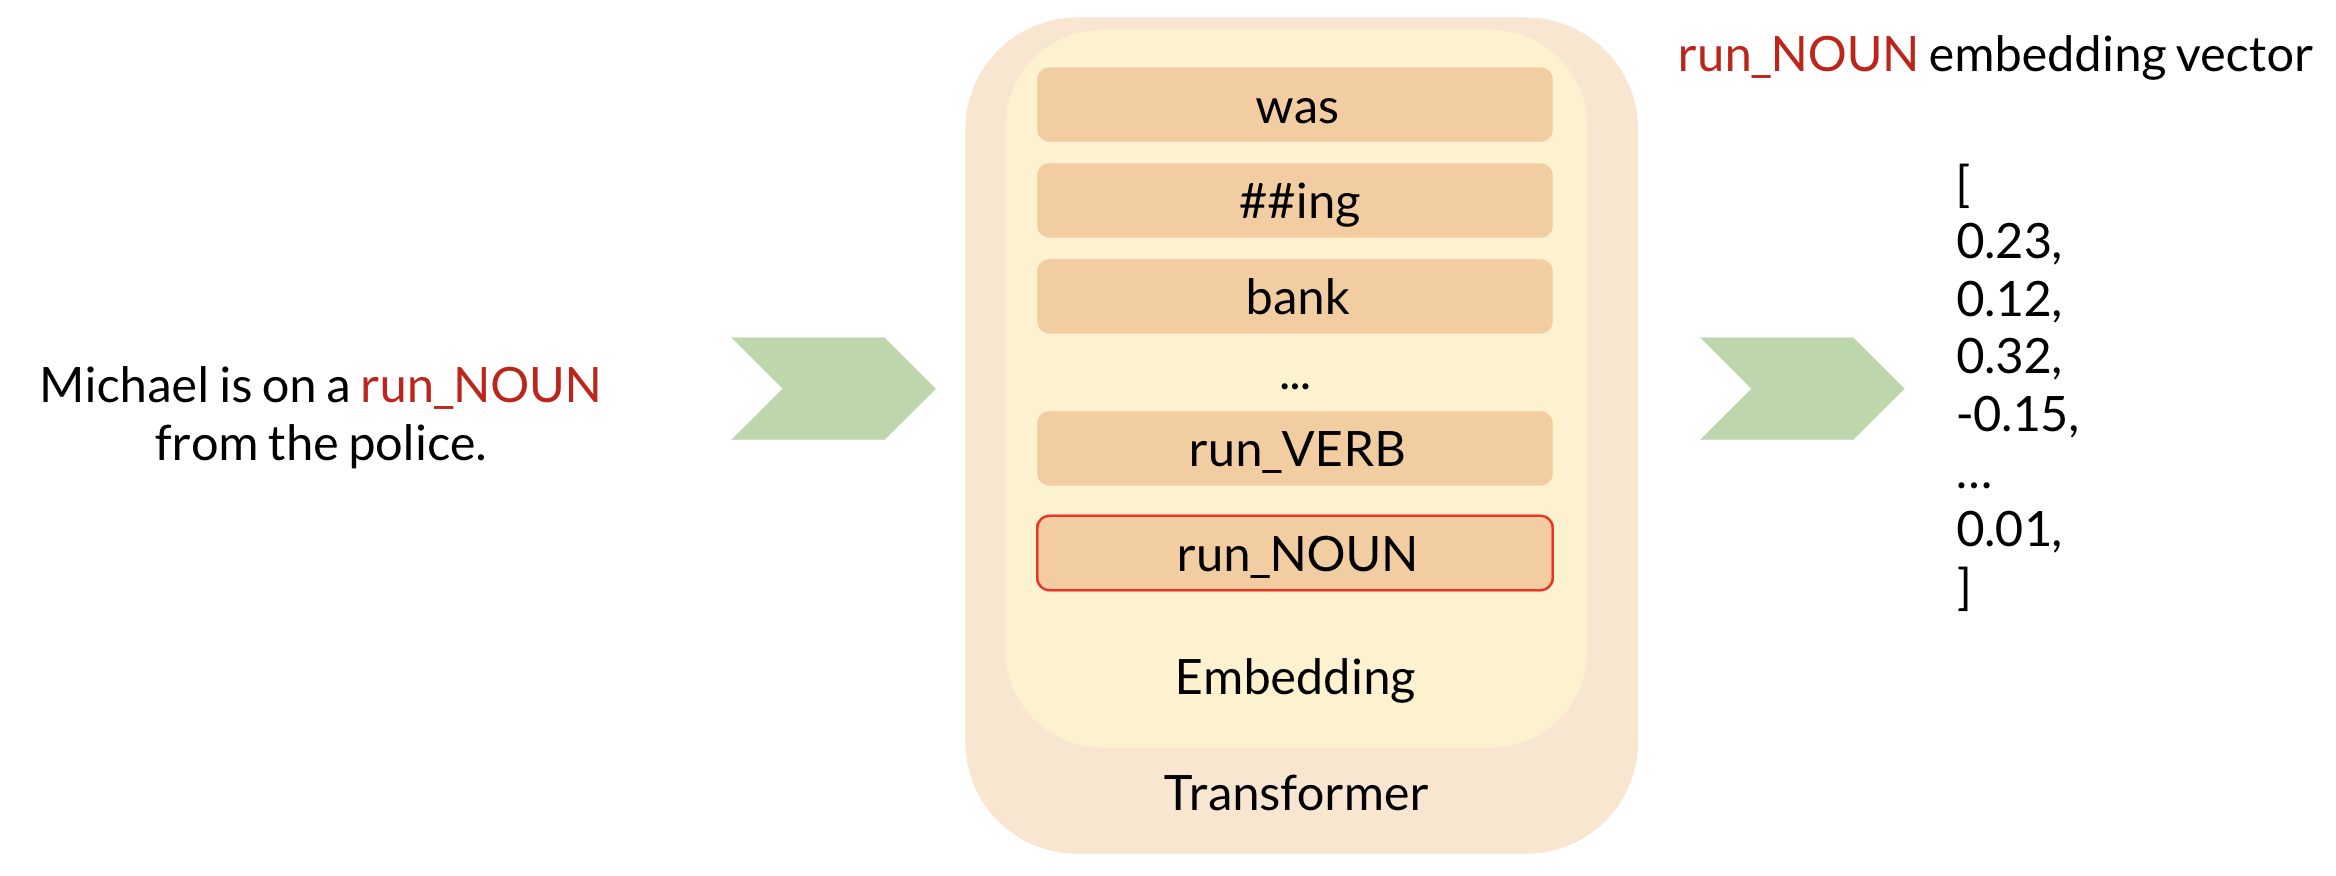
\includegraphics[width=\linewidth]{./assets/experiments/pipeline_tokenizer_BERnie_POS_input.png}
  \caption{}
  \label{fig:cbow_skipgram}
\end{figure}

\begin{figure}[h]
	\center
  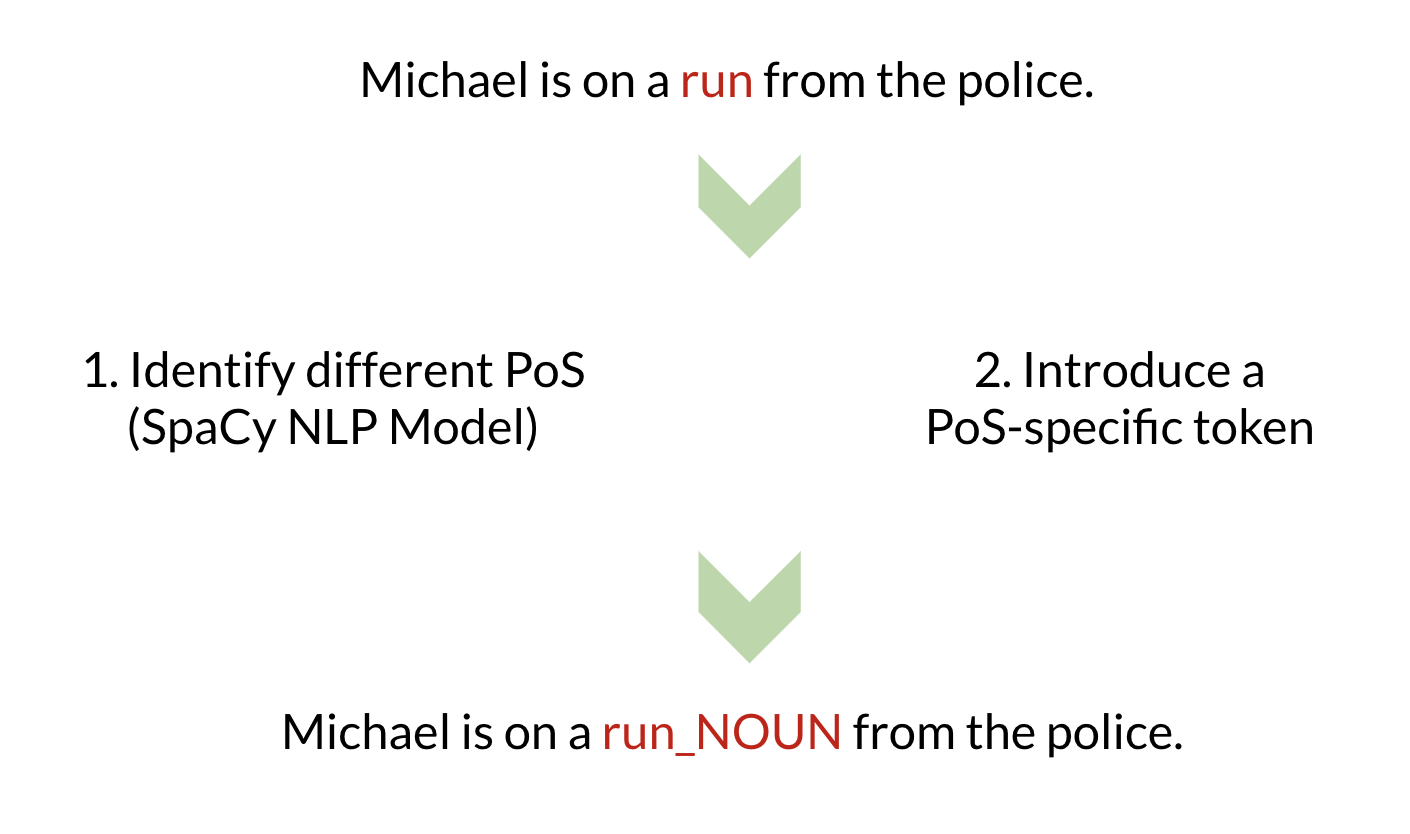
\includegraphics[width=\linewidth]{./assets/experiments/pipeline_tokenizer_BERnie_POS_sentence.png}
  \caption{}
  \label{fig:cbow_skipgram}
\end{figure}

\begin{figure}[h]
	\center
  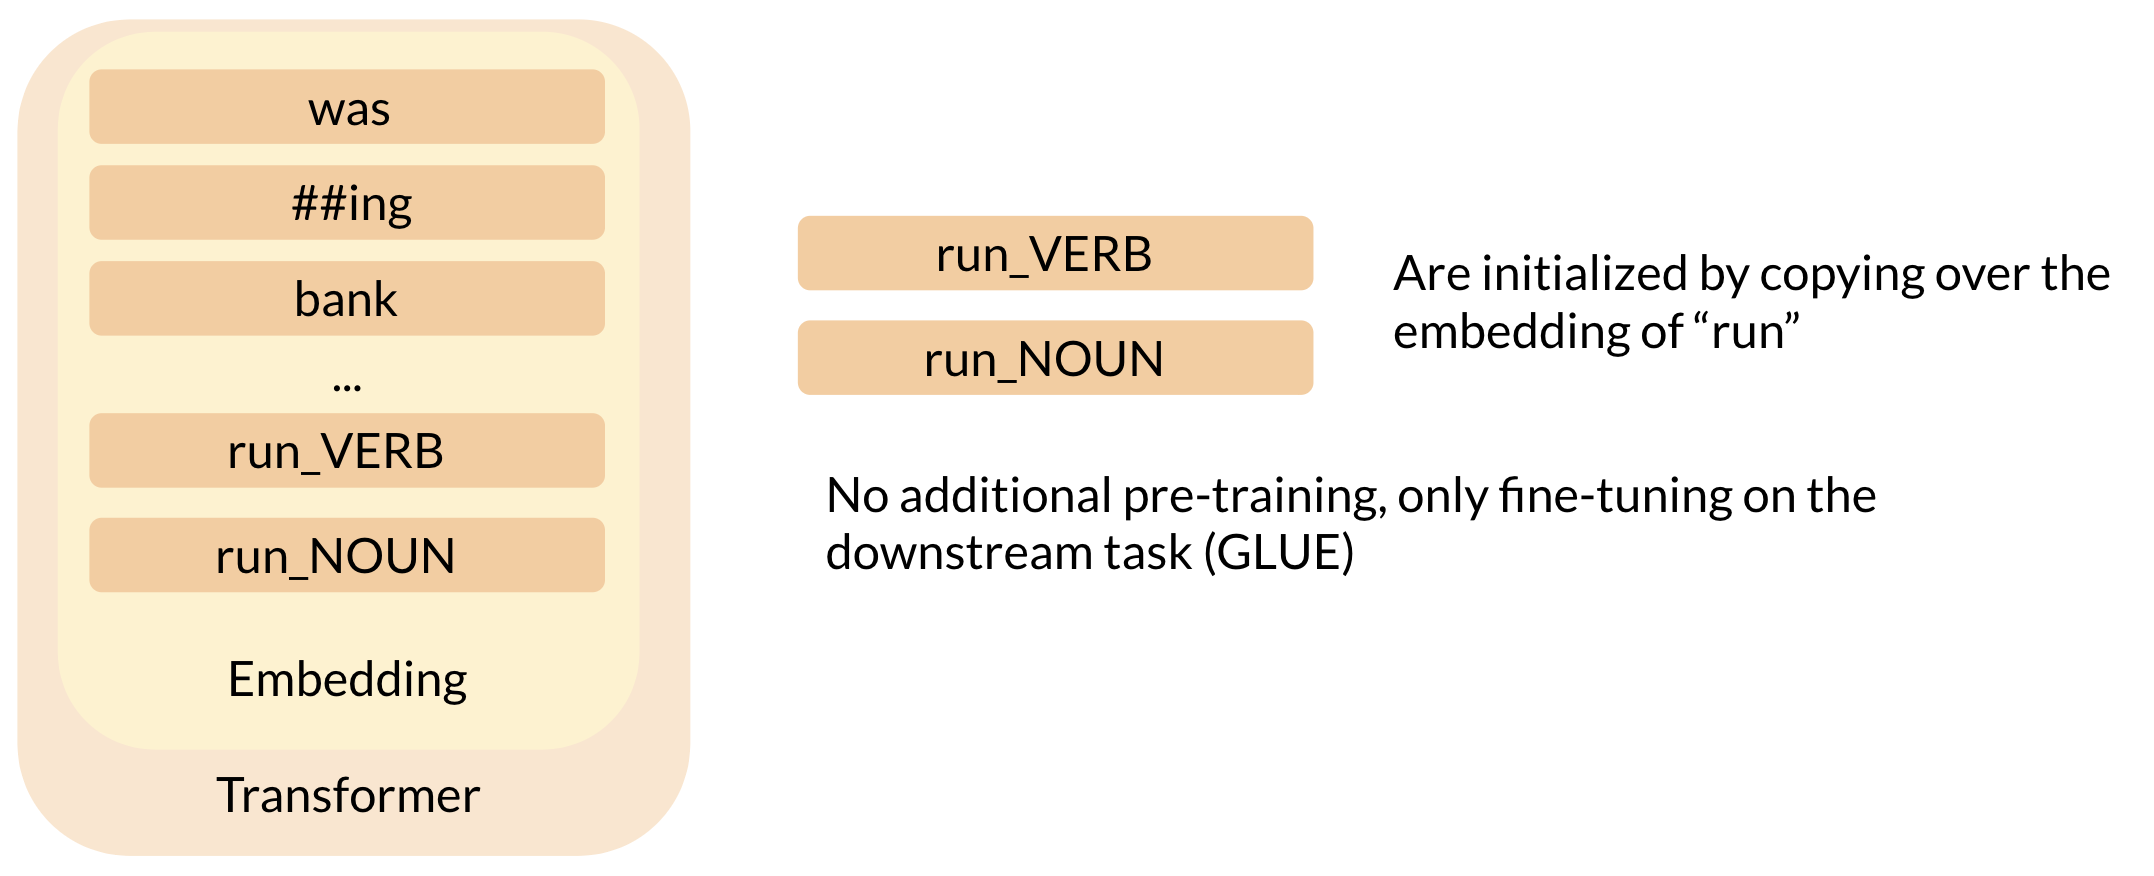
\includegraphics[width=\linewidth]{./assets/experiments/pipeline_model_BERnie_POS_initialization.png}
  \caption{}
  \label{fig:cbow_skipgram}
\end{figure}

\subsection{BERnie Meaning}

\subsubsection{Motivation}

\subsubsection{Experiment setup}

\begin{figure}[h]
	\center
  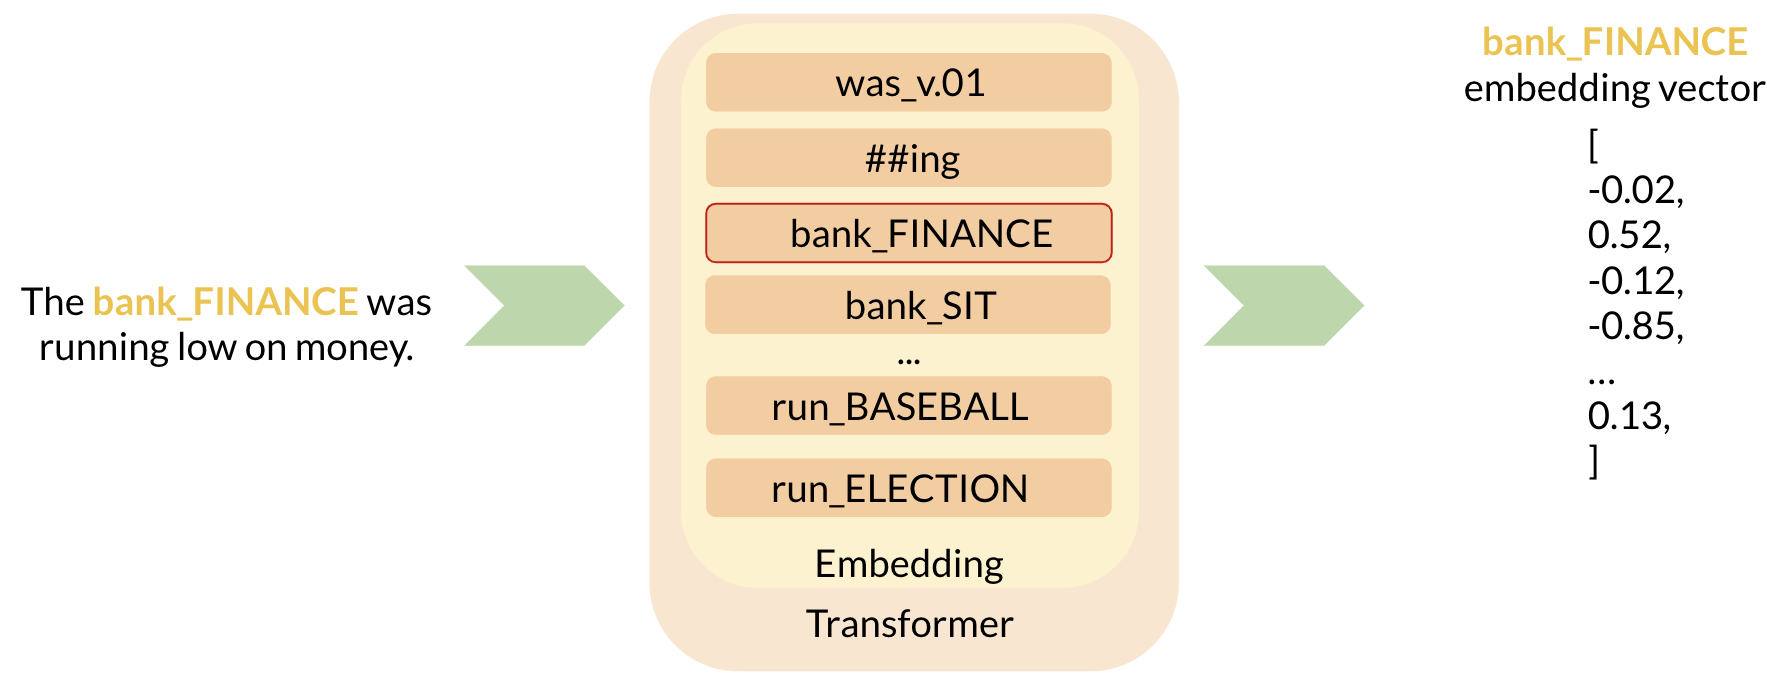
\includegraphics[width=\linewidth]{./assets/experiments/pipeline_model_BERnie_meaning.png}
  \caption{}
  \label{fig:cbow_skipgram}
\end{figure}


\begin{figure}[h]
	\center
  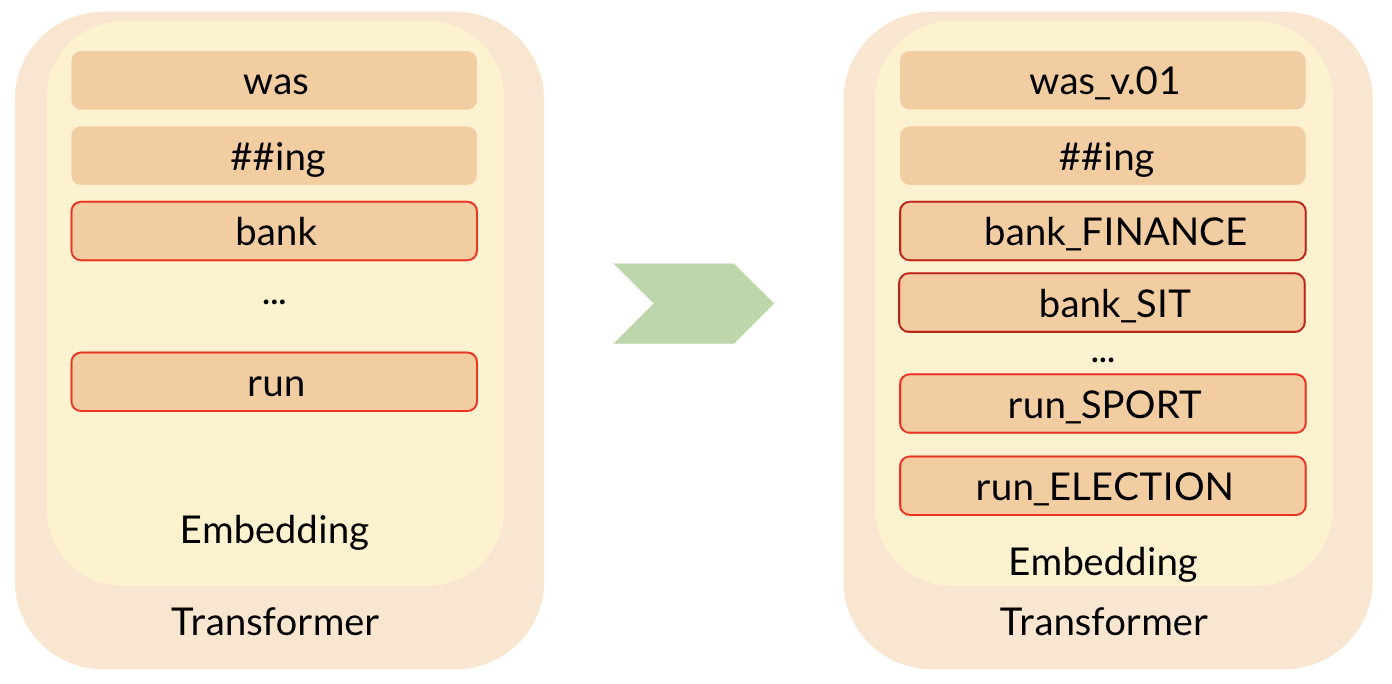
\includegraphics[width=\linewidth]{./assets/experiments/pipeline_model_BERnie_meaning_embedding.png}
  \caption{}
  \label{fig:cbow_skipgram}
\end{figure}


\begin{figure}[h]
	\center
  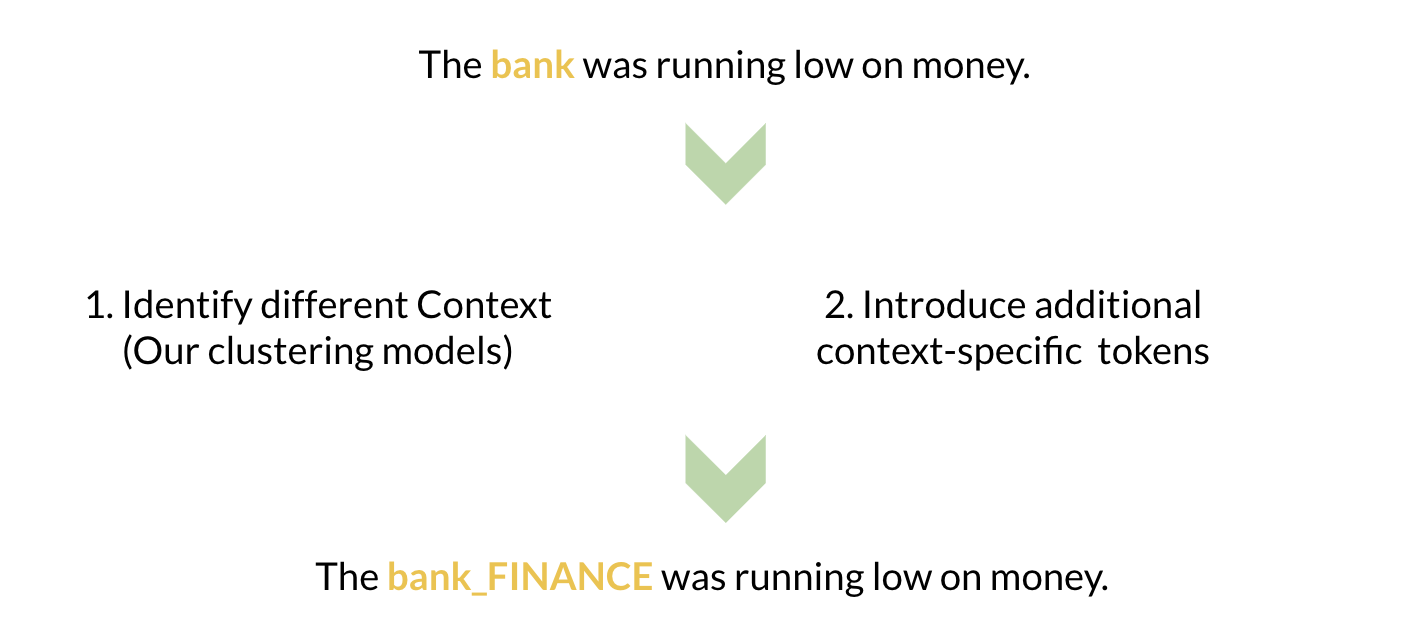
\includegraphics[width=\linewidth]{./assets/experiments/pipeline_tokenizer_BERnie_meaning.png}
  \caption{}
  \label{fig:cbow_skipgram}
\end{figure}


\begin{figure}[h]
	\center
  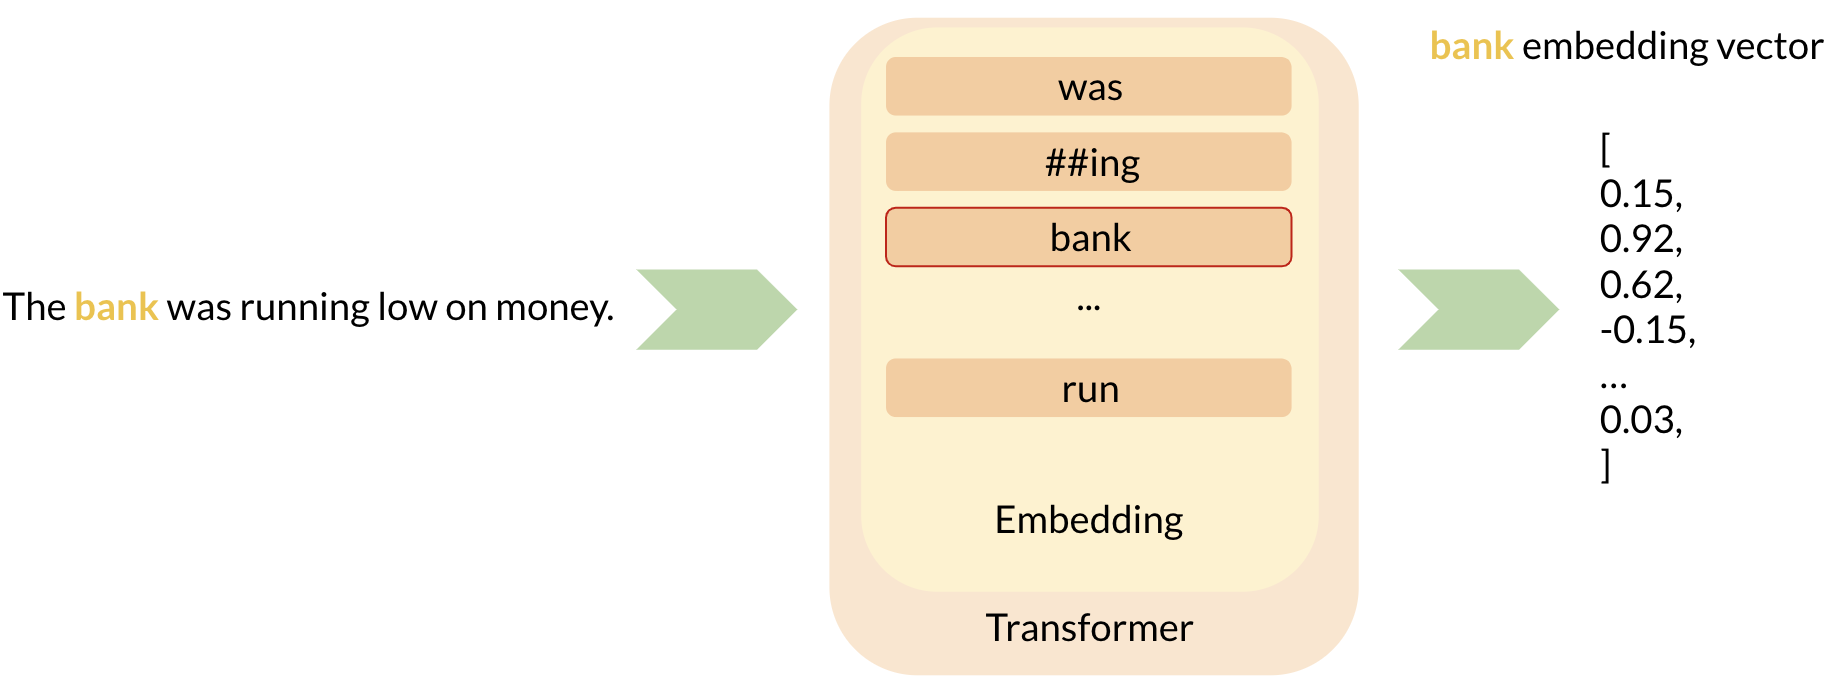
\includegraphics[width=\linewidth]{./assets/experiments/pipeline_tokenizer_BERnie_meaning_.png}
  \caption{}
  \label{fig:cbow_skipgram}
\end{figure}


\subsection{BERnie Meaning with additional pre-training}
\subsubsection{Motivation}
\subsubsection{Experiment setup}

\subsection{Compressing the non-lexical out}
\subsubsection{Motivation}
\subsubsection{Experiment setup}

\
%\chapter{Summary and Conclusions} 
\chapter{Evaluation}

We evaluate the models of the previous experiments.

\begin{center}
\captionof{table}{Mean and standard deviation of the accuracy of a linear classifier trained on the the 4 most common classes of WordNet meanings for the word \textit{was}.}
\begin{tabular}{SSSSSSSS} \toprule
    {dimensionality} & {variance kept} & {accuracy (mean / $\pm$ stddev)}  \\ \midrule
       2  & 0.08 & 0.38 / $\pm$ 0.03 \\ \midrule
       3  & 0.11 & 0.38 / $\pm$ 0.04 \\ \midrule
     10  & 0.28 & 0.65 / $\pm$ 0.03  \\ \midrule
     20  & 0.43 & 0.76 / $\pm$ 0.04  \\ \midrule
     30  & 0.53 & 0.83 / $\pm$ 0.03  \\ \midrule
     50  & 0.67 & 0.93 / $\pm$ 0.01 \\ \midrule
     75  & 0.77 & 0.95 / $\pm$ 0.01 \\ \midrule
    100 & 0.83 & 0.95 / $\pm$ 0.01  \\ \midrule
\end{tabular}
\end{center}

%TODO Write section for GLUE tasks
\scalebox{0.9}{
\begin{tabular}{
 l % left aligned column
 l % left aligned column
 *{5}{S[table-format=4.0]} % three columns with numeric data       
}
\toprule
%TODO MRPC has one aligned, and one unaligned test
&&\textbf{BERT} & \textbf{BERnie PoS} & \textbf{BERnie} \\
\midrule
CoLA  & Accuracy  &  \textbf{0.5739} & 0.5263 &  0.5457 \\

MRPC & Accuracy &  \textbf{0.8223} & 0.8199 &  0.8064 \\
          & F1           &  \textbf{0.8778} & 0.8614  &  0.8684 \\
          & Mixed     &  0.8501 & \textbf{0.8579}  &  0.8374 \\
          
SST-2 & Accuracy  &  0.9214 & 0.9203 &  \textbf{0.9266} \\

STS-B & Correlation &  \textbf{0.8841} & 0.8615 &  0.8574 \\
      & Pearson & \textbf{0.8860} & 0.8621         & 0.8587 \\
      & Spearman & \textbf{0.8822} & 0.8601      & 0.8567 \\
      
QNLI & Accuracy &  \textbf{0.9126} & 0.9090    &  0.9020 \\

RTE & Accuracy &  \textbf{0.6462} & 0.6083     &  0.5722 \\

WNLI & Accuracy &  0.35915 & 0.39465 &  \textbf{0.4649} \\

MNLI & Accuracy &  0.8453 &              &  0.8334 \\

SNLI & Accuracy &  \textbf{0.8461} &              &  0.8367 \\

QQP & Accuracy &  \textbf{0.9113} &              &  0.9042 \\
      & F1     & \textbf{0.8809} &                       & 0.8732 \\
      & Mixed & \textbf{0.8961} &                    & 0.8887 \\
      
\bottomrule
\end{tabular}
}

All values are the average of two runs. 
Weights which are instantiated specifically for the GLUE tasks are once instantiated with a random seed of 42, and once with a random seed of 101.

Although most experimental results are similar between standard BERT and the modified BERnie PoS and BERnie models, the WNLI and RTE experiments are considerably deviating in performance through the addition of the additional embedding vectors.
For the BERnie model, WNLI performs \textbf{10.56\%} better than standard BERT, and RTE performs  \textbf{-7.40\%} worse than the standard BERT implementation.
Similar results are observable for the difference between the unmodified BERT and the BERnie PoS model with \textbf{3.52\%} improvement for WLNI and \textbf{-3.79\%} decline in performance for the RTE task.

%TODO : Describe what kind of task WNLI is
%TODO : Describe what kind of task RTE is

%TODO we use the GLUE tasks to understanding how introducing more embedding vectors affects the performance of our search models.


To train an ablation study, whether or not additional pre-training improves the instantiated word-vectors, we conduct the following experiment.
We instantiate the additional embeddings as described in the previous section.
We then run one full epoch of training with the same training parameters as used for GLUE on the news.corpus.2007 dataset using a masked languag emodel methodology .
%TODO cite BERT training methodology
We save this model and load it for the GLUE tasks.
BERnie full Pre-training trains the entire embeddings, whereas BERnie partial Pre-Training fixates all embedding vectors except the ones for the ones that were newly added.

%TODO Write section for GLUE tasks
\scalebox{0.9}{
\begin{tabular}{
 l % left aligned column
 l % left aligned column
 *{3}{S[table-format=4.0]} % three columns with numeric data       
}
\toprule
%TODO MRPC has one aligned, and one unaligned test
&& \textbf{BERnie} & \textbf{BERnie full\- Pre}  & \textbf{BERnie partial\- Pre}\\
\midrule
CoLA  & Accuracy  &  0.5457 & 0.5418 & 0.5731 \\
MRPC & Accuracy &  0.8064 & 0.3824 & 0.3162\\
          & F1           &  0.8684 & 0.1720 & 0.0000 \\
          & Mixed     &  0.8374 & 0.2775 & 0.1581 \\          
SST-2 & Accuracy  &  0.9266 & 0.9169 & 0.9266 \\
QNLI & Accuracy & 0.9020 & 0.5374 & 0.6700 \\
RTE & Accuracy &  0.5722 & 0.4784 & 0.4729 \\
WNLI & Accuracy & 0.4649 & 0.4225 & 0.4507 \\
\bottomrule
\end{tabular}
}

\chapter{Conclusion}

\appendix
\singlespacing

\bibliographystyle{unsrt} 
\bibliography{dissertation} 

\end{document}
